
\chapter{Results}\label{chap:4}
% \section{Prototyping/Evaluating the System}
% 5-7 pages
% \lipsum[1]\todo{TODO}


    
This chapter will provide an overview of the achieved results, the determined baselines, the setup of the experiments, the nature of the environment and the experiment process to solve the posed research question. 
This chapter also adapts the structure for machine learning algorithms proposed by \textcite{luckert2016using}.
%  the pipeline deployment details,  collection and labelling steps, the neural network implementation and training. Finally, the pose estimation algorithms and the pipeline are evaluated.
Section \ref{chap:4:setup} illustrates the environment and sensors setup, 
section \ref{chap:4:behaviors} describes the exploration and voxel-curious behaviors setup, 
% section \ref{chap:4:train_data} explains the data collection and neural network training, 
% section \ref{chap:4:\ref{chap:4:training}} detailing the training , 
and section \ref{chap:4:results} presents the experiment results. The following questions will be answered thoroughly:
\begin{itemize}
    \item How were the experiments set up?
    % \item What was the cloud deployment setup for the solution?
    \item How many episodes, metrics, etc., were ran and collected for training, testing and optimizing the algorithms?
    % \item Which tools were used to acquire the metrics, create the data and perform the experiments?
    \item Which algorithm parameters were the most influential?
    % \item Which algorithm optimizations were done?
    \item What were the achieved results on each experiment?
    \item What was the setup of the best performing algorithm?
    % \item Which algorithm optimizations were done?
\end{itemize}

As we approach the presentation of our results, it is important to step back for a moment to look at our approach from two perspectives. The initial presented perspective looks at the problem as an object uncertainty problem, where our interest is to look at objects from multiple perspectives to reduce our \textit{uninformativeness} about them. To this end, we proposed a reinforcement learning agent that explores environments to find such objects of interest.
However, the second perspective for our proposed method is a navigation perspective, which was implicitly presented through our related works. As mentioned before, visual navigation solutions can be categorized depending if the location of the goal is known or unknown \cite{chaplot2020semantic}. Among these, the commonly studied point-to-goal task presents two fallacies
\begin{itemize}
    \item the location of the goal is known (either implicitly through a path or explicitly through coordinates), which is not the case in, for example, rescue missions.
    \item the goal is not situated very far from the target (exhaustive exploration is not required), which conceals the real exploratory performance of embodied algorithms.
\end{itemize}

Not only do traditional navigation approaches depend on map awareness, to subsequently execute some sort of path-planning algorithm, but real life problems such as rescue scenarios or dynamic environments, provide the agent with limited, changing, partial observability of the environment. This has laid the path for mapless solutions to take over classical navigation approaches \cite{mapslessETH, brandenburger, snapnav}. Our approach takes this into consideration to account for the partial observability in an unknown environment, where the location of goals are also unspecified.

Moreover, traditional approaches subdivide the navigation problem into sub-modules for obstacle avoidance, map creation and then path planning. Accordingly, newer approaches avoid the pitfalls of traditional, complex model-based approach which attempt to model the dynamics of the real world and carry some sort of bias. They also solutions leverage deep learning methods to provide end-to-end solutions to the navigation problem \cite{wang, maplessETH}. We therefore proposed a model-free method that leverages neural networks and that is capable of adapting across environments.  

All of these methods, however, usually depend on the quality of the sensorial data obtained to reconstruct the world to be navigated.
Dense mapping systems are usually victims of noise, outliers and missing data, and must even balance runtime performance and reconstruction quality. Moreover, these methods either ignore moving targets or use expensive raycast operations to construct maps of the dynamic objects in the scene. \cite{mapless, margarita} % of surfel clouds or TSDF Volumes 
This is the pinnacle for this thesis, where we propose the usage of voxels to provide our agent with robustness to outliers, noise and missing data, and octrees for the efficient, mapless, exploration of changing environments. 
Furthermore, we take inspiration from the physiology of pigeons' biological compass to provide our agent with a mapless technique to orient itself in unknown environments.
% , achieving 100% coverage of open world scene

Finally, as mentioned before, given the increasing momentum of reconstruction methods and synthetic data to fuel other machine learning pipelines \cite{plenoxels, nvidia}, we decided to exploit Unity 3D to train and test our agent in multiple 3D environments. This allows direct portability and extensibility of our agent to new methods, new scenarios, further benchmarks, etc. 
Without further delay, the following sections present the behavior setup for each agent variant, the of the training, and the results of the DARPA test environments.


% As presented in Section \ref{chap:3:further-use:evaluation-framework}, we test agents on 3D environments inspired by the DARPA-subterreanean challenge \cite{DARPA}, our method achieves a better performance by at least a factor of 2 in time-to-discovery in an open world environment of 160 m2, compared to our implementations of model-free shortest path methods, object-detector-based methods and semantic-curiosity-based methods. Where traditional methods achieve either navigation or trajectory planning around objects, our agent achieves model-free exploration of both objects and environments using efficient data structures in a mapless fashion.

% This, along the lines of 

% Our approach converges these two stories, since 
% It is of special interest to demonstrate that larger environments reveal weaker policies. Several works in navigation 

% different performance, as 



\section{Environment and Vision Setup}\label{chap:4:setup}

% As proof of concept for the project the test environment that was set up consisted of an artificial cow at the ZHAW and a robotic arm as shown by Figure \ref{fig:cow_setup}. The hardware setup for such an environment consisted of the following:


To carry out the experiments, a set of learning environments were required to train, collect metrics and test the different agent behaviors. These behaviors derivated as a result of different observations, hyperparameters, policies and reward signals. The implemented 3D environment is illustrated in Figure \ref{fig:unity-island}, with the respective exploration boundaries that limit the exploration space for the agent.

\begin{figure}[!ht]
    \centering
    \subfigure{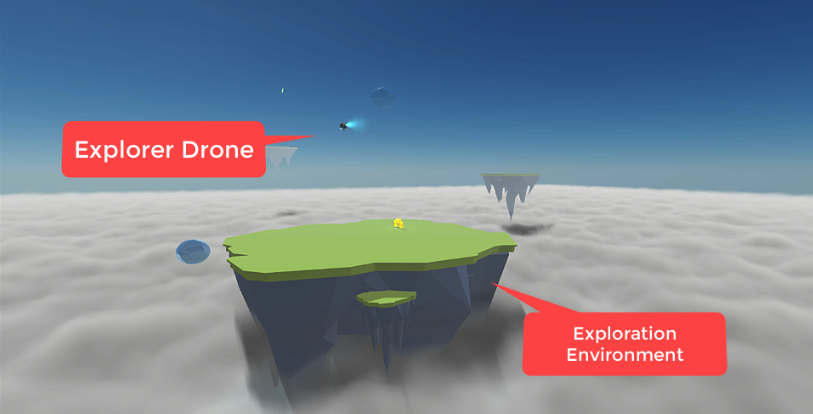
\includegraphics[width=0.49\textwidth]{images/unity-chapter4-intro.png}} 
    \subfigure{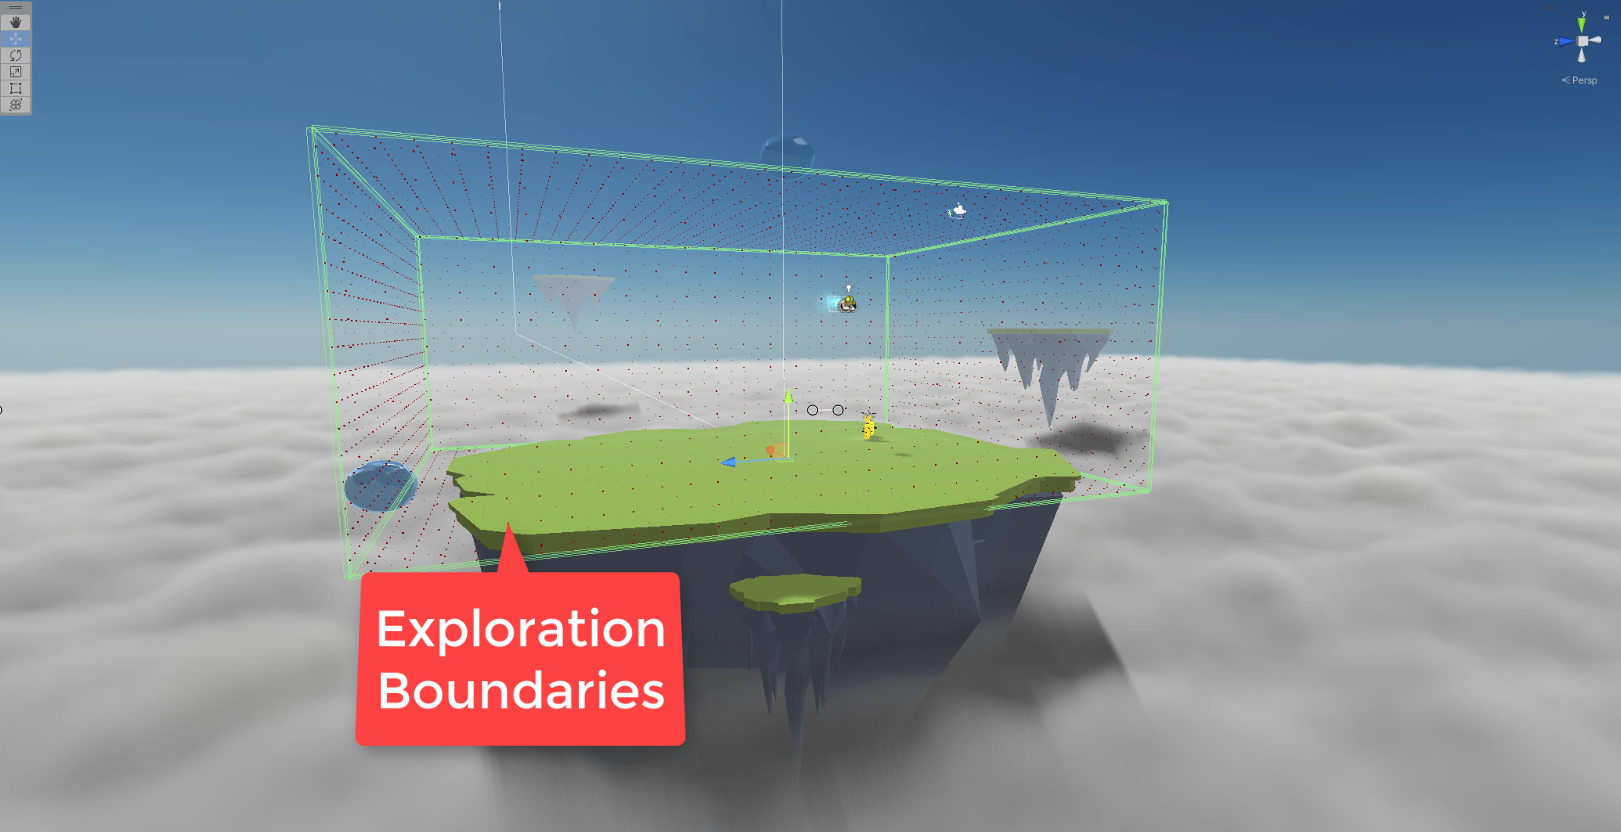
\includegraphics[width=0.49\textwidth]{images/unity-environments-training-boundaries.png}} 
    \caption{Training 3D environment in Unity 3D with explorer drone (left). Exploration boundaries of training environment to delimit evaluation zone (right). Created using 3D models from \cite{unity-asset-store}.}
    \label{fig:unity-island}
\end{figure}

% 
% are voxelized and a reinforcement learning agent explores an environ
% % Tasks
% % in this category do not require exhaustive exploration of the environment as the
% % location of the goal is known explicitly (coordinates) or implicitly (path).
% Visual Navigation and Exploration. Prior work on visual navigation
% can broadly be categorized into two classes based on whether the location of the
% goal is known or unknown. Navigation scenarios, where the location of the goal is
% known, include the most common pointgoal task where the coordinate to the goal
% is given [26,40].
% In point-to-goal tasks two irrealistic things occur:

% It is of spAs claimed by [ref], many exploration approaches shoot themselves in the foot by using methods that rely on heavy data structures in the form of point clouds, meshes, etc., which limits area they can explore.
% Other methods do not consider the efficiency problem at all and are short-sighted to scenarios where the goal is a couple steps ahead of the agent's starting point. 
To analyze changes in performance given a larger training environment, we compare the agents' performance across a \textit{small} environment of 32 $m^2$ and a \textit{large} environment of 160 $m^2$. Figure \ref{fig:unity-islands-bigsmall} shows the two variants of the established 3D environment, where the large environment also includes obstacles for the agent to navigate around.


\begin{figure}[!ht]
    \centering
    \subfigure{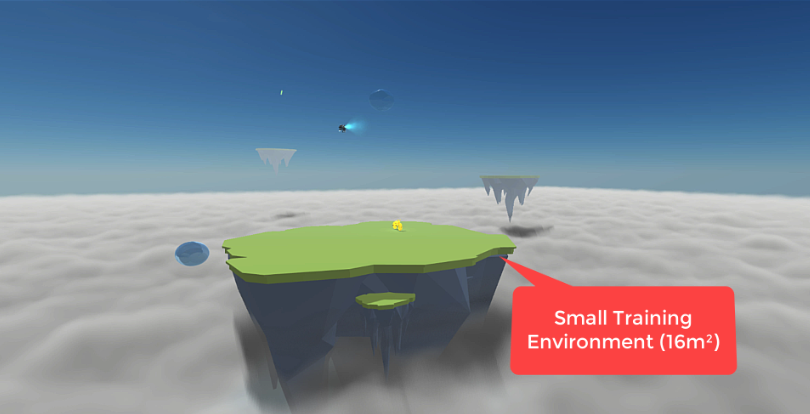
\includegraphics[width=0.49\textwidth]{images/unity-chapter4-small.png}} 
    \subfigure{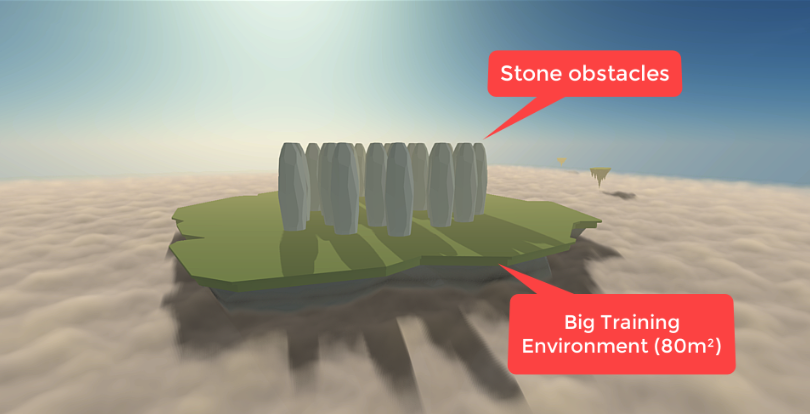
\includegraphics[width=0.49\textwidth]{images/unity-chapter4-big.png}} 
    \caption{Sample 3D assets for scenario proposals. Taken from \cite{unity-asset-store}.}
    \label{fig:unity-islands-bigsmall}
\end{figure}

Consequently, after the definition and setup of the environment, the next step is the setup of the vision system. As described in more detail in the previous chapter, the approach to perception was to use the grid sensors from \cite{github-unity-mlagents-toolkit, github-mbaske-gridsensor}. 
% These grid sensors create a mesh of ray casts that mimic the output of a normal depth camera to interpret an abstracted view that takes the form of simplified, voxelized view of the environment. As also mentioned in the previous chapter, their output is then fed through a visual encoder that uses convolutional neural networks to transform this visual input for the agent. 
Figure \ref{fig:unity-island-gridsensors} visualizes the range of the two grid sensors used in the agent and the voxelized view they produce. 
At the implementation level, the unwrapping of the grid sensor input into the 3D grid shown in Figure \ref{fig:unity-island-gridsensors} is done through multiple Unity box colliders at each grid cell. 
The detected objects at each collider are then mapped to a position in a matrix which are then input to the simple encoder and also displayed in the Unity UI. For more technical information on the implementation of the grid sensor please refer to \cite{github-mbaske-gridsensor}.

One grid sensor is used to visualize elements in a panoramic fashion within a radius of 16 meters, where elements of three types are detected: boundaries, obstacles and collectibles.
A second and smaller grid sensor with a diameter of 6 meters acts as the scanner in the voxel-exploration task: this grid sensor mimics a "scanneable" area and has a fail-rate of 20\% to provide the agent with an imperfect scanning behavior. Voxels that fall into this grid sensor's area are marked as scanned and accumulated by a counter to reward the agent at timestep \textit{t}. 

\begin{figure}[!ht]
    \centering
    \subfigure{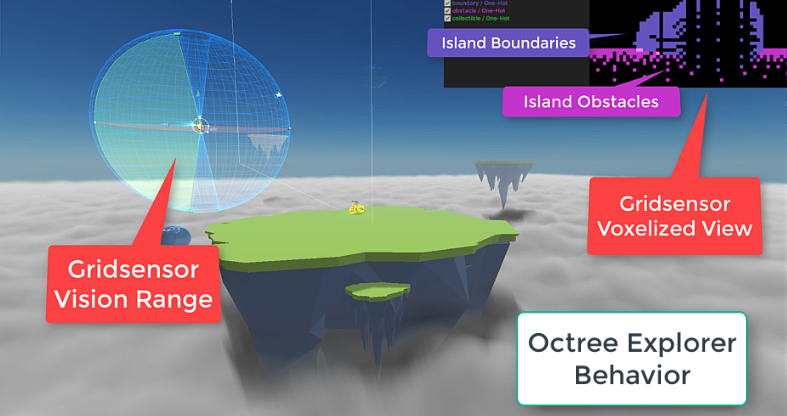
\includegraphics[width=0.49\textwidth]{images/unity-environments-training-gridsensor-single-octree.png}}
    \subfigure{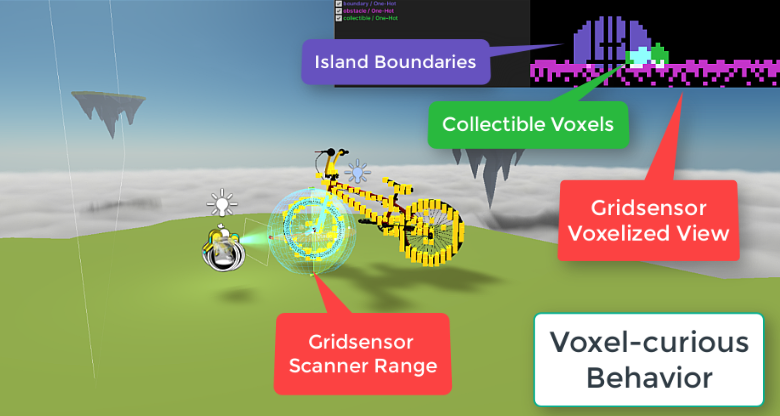
\includegraphics[width=0.49\textwidth]{images/unity-environments-training-gridsensor-single-voxel.png}} 
    \caption{Integrated grid sensor used for the agent to perceive objects, boundaries and collectibles (left). Grid sensor used by the agent as a voxel-scanner (right). Voxelized-view perceived through the grid sensors is also shown.}
    \label{fig:unity-island-gridsensors}
\end{figure}

% \newpage 
 
\section{Behaviors Setup}\label{chap:4:behaviors}

The setup of the agent behaviors for the exploration of octrees and voxels is comprised by the set of observations and rewards provided to motivate a certain policy. The octree exploration policy was motivated by the approach presented by \textcite{chen2019learning}, where each discovered node in the octree provides a certain reward to the agent. To analyze the behavior of different octree setups, diverse experiments were run with varying from nodes of 4 $m^3$ to 16 $m^3$. Therefore, the rewarding styles for octree exploration policies vary according to the size of the octree nodes the agent can discover.


\begin{figure}[!ht]
    \centering
    \subfigure{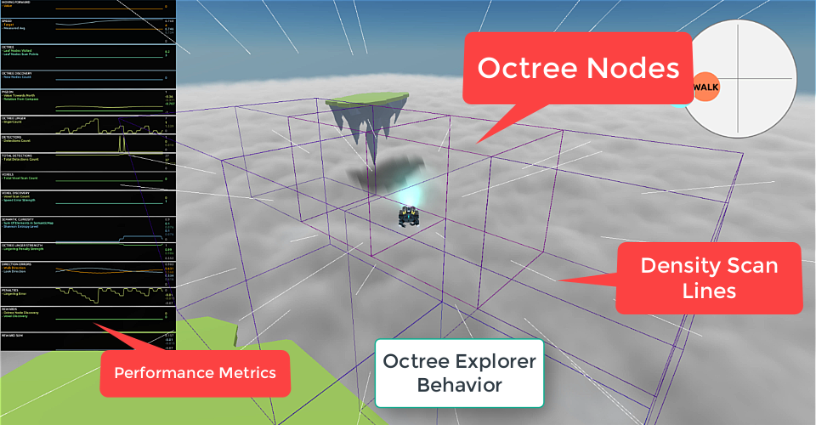
\includegraphics[width=0.49\textwidth]{images/unity-environments-training-behavior-octree2.png}} 
    \subfigure{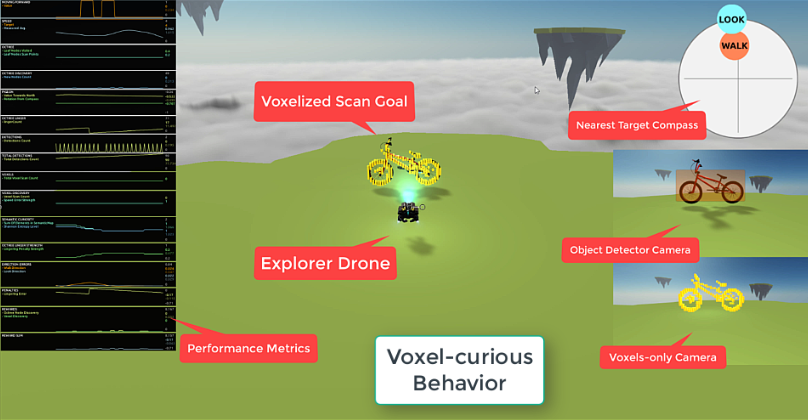
\includegraphics[width=0.49\textwidth]{images/unity-environments-training-behavior-voxel.png}} 
    \caption{Sample 3D assets for scenario proposals. Taken from \cite{unity-asset-store}.}
    \label{fig:unity-my-3d-envs}
\end{figure}


A second branch of variants of this approach take into account something called \textit{pigeon observations}. These observations take inspiration of the physiology used by pigeons to orient themselves in their environment, memorize routes and keep a biological compass. They consist of two vectors: one towards a geographical north and one towards a sun placed on top of the training island. 

Finally, following the example given by \textcite{chaplot2020semantic}, we analyze the performance of a "blind" octree variant that is curious for new states following the approach proposed by  \textcite{pathak2017curiosity} and then compare it to the octree methods that follow \textcite{chen2019learning}'s approach. Moreover, as motivated by \textcite{github-unity-mlagents-toolkit}, we go one step further and integrate \textcite{pathak2017curiosity}'s parameters into the agent's model to construct our proposed explorer drone, which takes into account all three: 1) octree observations, 2) pigeon observations and 3) pathak's curiosity for new states. In summary, in addition to the information presented about the choice of agent observations in Section \ref{chap:3:agent-choice-actions} and the baseline agents in Section \ref{chap:3:interpretation}, the diverse setups for environment-focused agents are a combination of the following:

\begin{itemize}
    \item Agents with a reward for discovering 4-, 8-, 16-meter-wide octree leaf nodes.
    \item Agents with one or more of the following environment observations:
    \begin{itemize}
        \item Amount of octree nodes discovered at timestep $t$.
        \item Pigeon observations.
        \item Lingering factor.
    \end{itemize}

    \item Agents penalized given their lingering behavior.
    \item Agents with Pathak's curiosity module (main feature of the \textbf{Pathak} baseline agent).
    \item Agents with a minimum speed penalty.
\end{itemize}

It is worth clarifying that \textbf{blind} octree agents receive a reward for discovering new nodes but do not receive any of the aforementioned observations. Furthermore, mentioned in Section \ref{chap:3:interpretation}, Pathak's method was initially proposed for the exploration of environments but is now incorporated as a curiosity module


Similarly, the voxel exploration policy was motivated by a rewards-per-voxel fashion, where the diverse policies vary according to the reward per voxel, ranging from a 25\% reward per voxel to a 100\% reward per voxel. 
The diverse setups for object-focused agents are a combination of the following:
\begin{itemize}
    \item Agents with a reward for discovering a voxel with a reward by a factor in the range: 25\%, 50\%, 75\%, and 100\%.
    \item Agents with, alternatively, a normalized voxel reward given by $ R^{VOX} = \frac{voxels\_scanned}{2 + voxels\_scanned} $.
    \item Agents with one or more of the following environment observations:
    \begin{itemize}
        \item Vision of voxels in the grid sensor.
        \item Lingering factor.
        \item Pigeon observations.
        \item Walk and look angles towards nearest object (main feature of \textbf{oracle} agents and the \textbf{shortest-path} baseline agent).
        \item Number of classes detected by the object detector (main feature of the \textbf{object detector} baseline agent).
        \item Rationalized class entropy (main feature of the \textbf{semantic curiosity} baseline agent).
        \item Lingering penalty strength (observed and regulated in our \textbf{voxel-entropy} agent).
        % \item Number of classes detected by the object detector (main feature of the object detector baseline agent).
    \end{itemize}
    \item Agents with a minimum speed penalty.
    \item Agents with a lingering penalty.
    % \item Agents penalized given their lingering behavior.
\end{itemize}

Each agent behavior presented in the following sections was trained for \textbf{30 million timesteps} using PPO and variations of the hyperparameters presented in \ref{appendix:ppo-trainer}. Following the 80-20 rule, test runs had a duration of 7.5 million timesteps. 
Tables \ref{appendix:baselines_observations}, \ref{appendix:baselines_rewards} present a complete overview of the different agent variants trained. 


% \newpage

\section{Results}\label{chap:4:results}
This section presents the results of the experiments. Section \ref{chap:4:results-RQ2} deals with the results concerning the exploration of objects and \ref{chap:4:results-RQ1} deals with the results concerning the exploration of unknown spaces using octrees. Each subsection will present the best results obtained on the exploration policy variants and a brief description of the most representative details of each variant.

% • How can an embodied agent increase the overall certainty about an object’s characteristics, i.e., how
% can trajectories around objects of interest be generated to reduce the uncertainty about such objects?
% • How can these objects be found in large and unknown environments by the same agent

\subsection{Research Question 1}\label{chap:4:results-RQ1}

The first research question focuses on the reduction of uncertainty about objects, which we have posed as a voxel-curiosity task. Below, the best results for each voxel-curious variant are be presented in two subsections according to if the model has knowledge of voxels. 
It is worth mentioning that the training environment provided the agent 6 goals per episode situated at a distance of 5-50 meters away from the origin. 
In contrast, the DARPA testing environment contained a single goal located between 30 to 50 meters away from the origin. This sparse-reward testing environment evaluates the actual explorative capabilities of an agent.
For information on the run names, please refer to the previous Section \ref{chap:4:behaviors} and Appendix \ref{appendix:agents_explanations}.


% \newpage

\subsubsection{Agents with Knowledge of Voxels}
The following Table \ref{tab:RQ1-results} shows a brief overview of the results at the top 50 percentile based on the average amount of objects scanned. More information about all methods are presented in the tables afterwards.
\begin{longtable}{|l|c|c|}                            \hline %c|
    % \multicolumn{3}{|l|}{\textbf{Voxel-Curiosity}}              \\\hline
    \theadcenteredLeft{Method}            
    & \theadcentered{Episode Length \%}                
    & \theadcentered{Average Total Objects Scanned}  \\ \hline
    % & \thead{Standard Deviation}            \\ \hline
    % run61-voxel	&	100	\%	&	0.34	&	0.10	\\ \hline
    % run61-voxel-constrained	&	100	\%	&	0.33	&	0.11	\\ \hline
    % run63++025	&	89	\%	&	1.56	&	0.24	\\ \hline
    % run63++050	&	94	\%	&	1.05	&	0.20	\\ \hline
    % run63++075	&	71	\%	&	0.96	&	0.17	\\ \hline
    % run63++100	&	99	\%	&	0.77	&	0.17	\\ \hline
    % run63++100-nospeed	&	97	\%	&	1.52	&	0.20	\\ \hline
    % run63++100-nospeed-nolinger	&	98	\%	&	1.73	&	0.21	\\ \hline
    % run63-normalized	&	97	\%	&	0.40	&	0.22	\\ \hline
voxel++025 & 94 & {\cellcolor[HTML]{B6D8D1}} \color[HTML]{000000} 1.56 \\ \hline
voxel++100-nospeed & 98 & {\cellcolor[HTML]{BEDCD6}} \color[HTML]{000000} 1.52 \\ \hline
voxel++100-nospeed-nolinger & 97 & {\cellcolor[HTML]{98CAC0}} \color[HTML]{000000} 1.73 \\ \hline
voxel++100-nospeed-nolinger-oracle & 96 & {\cellcolor[HTML]{E0EDEA}} \color[HTML]{000000} 1.33 \\ \hline
voxel++100-nospeed-nolinger-oracle-8 & 99 & {\cellcolor[HTML]{90C6BB}} \color[HTML]{000000} 1.77 \\ \hline
voxel++100-nospeed-nolinger-pigeon-oracle-8 & 97 & {\cellcolor[HTML]{E6F0EE}} \color[HTML]{000000} 1.30 \\ \hline
voxel++100-nospeed-oracle-4 & 100 & {\cellcolor[HTML]{A9D2CA}} \color[HTML]{000000} 1.64 \\ \hline
voxel++100-nospeed-oracle-8-pigeon & 93 & {\cellcolor[HTML]{A1CFC5}} \color[HTML]{000000} 1.68 \\ \hline
object-detector-pure-vision & 99 & {\cellcolor[HTML]{BADBD4}} \color[HTML]{000000} 1.54 \\ \hline
voxel-entropy++100-nospeed & 97 & {\cellcolor[HTML]{55AA99}} \color[HTML]{000000} 2.10 \\ \hline
voxel-entropy++100-oracle & 96 & {\cellcolor[HTML]{EBF2F0}} \color[HTML]{000000} 1.27 \\ \hline
voxel-entropy++100-oracle-nospeed & 98 & {\cellcolor[HTML]{B1D6CE}} \color[HTML]{000000} 1.59 \\ \hline


    \caption{Overview of the best object-focused runs with knowledge of voxels respect to the \textit{Episode Length} and the \textit{Total Objects Scanned} metrics. A small episode length indicates that the agent is overwhelmed by the penalties and the fastest way to minimize the reward function is to end the episode. An object is marked as scanned once all voxels that belong to it are scanned by the agent.
    } \label{tab:RQ1-results}
\end{longtable}

% \newpage
Table \ref{tab:results-RQ1-walkLook} shows the results of relevant object-focused agents that are aware of voxels, using the total detections, the walk error and the look error. These last two errors represent the directional error to the nearest target for the agent; an agent may walk towards a target but look in another direction.
%  for the total of voxels scanned and also their performance measured by the amount of \textit{total detections}, the \textit{walk error} and the \textit{look error}
\begin{longtable}{|l|c|c|c|}                            \hline
    % \multicolumn{3}{|l|}{\textbf{Walk Error}}              \\\hline
    \theadcenteredLeft{Method}            
    & \theadcentered{Total Detections Count} 
    & \theadcentered{Walk Error} 
    & \theadcentered{Look Error}   \\ \hline
voxel & 610597.65 & {\cellcolor[HTML]{EAF2F0}} \color[HTML]{000000} 0.48 & {\cellcolor[HTML]{CBE3DD}} \color[HTML]{000000} 0.42 \\ \hline
voxel++025 & 426601.17 & {\cellcolor[HTML]{E0EDEA}} \color[HTML]{000000} 0.46 & {\cellcolor[HTML]{AAD3CB}} \color[HTML]{000000} 0.37 \\ \hline
% voxel++050 & 426814.30 & {\cellcolor[HTML]{EBF2F0}} \color[HTML]{000000} 0.48 & {\cellcolor[HTML]{EBF2F0}} \color[HTML]{000000} 0.47 \\ \hline
% voxel++075 & 377998.18 & {\cellcolor[HTML]{E4EFEC}} \color[HTML]{000000} 0.47 & {\cellcolor[HTML]{E2EEEB}} \color[HTML]{000000} 0.46 \\ \hline
% voxel++100 & 360373.23 & {\cellcolor[HTML]{E3EEEC}} \color[HTML]{000000} 0.47 & {\cellcolor[HTML]{D9EAE6}} \color[HTML]{000000} 0.44 \\ \hline
voxel++100-nospeed & 315159.74 & {\cellcolor[HTML]{E2EEEB}} \color[HTML]{000000} 0.46 & {\cellcolor[HTML]{C7E1DB}} \color[HTML]{000000} 0.41 \\ \hline
voxel++100-nospeed-nolinger & 425433.05 & {\cellcolor[HTML]{E5EFED}} \color[HTML]{000000} 0.47 & {\cellcolor[HTML]{C5E0DA}} \color[HTML]{000000} 0.41 \\ \hline
voxel++100-nospeed-nolinger-oracle & 487909.34 & {\cellcolor[HTML]{D0E5E1}} \color[HTML]{000000} 0.43 & {\cellcolor[HTML]{C4E0DA}} \color[HTML]{000000} 0.41 \\ \hline
% voxel++100-nospeed-nolinger-oracle-8 & 322132.54 & {\cellcolor[HTML]{C7E1DB}} \color[HTML]{000000} 0.41 & {\cellcolor[HTML]{CBE3DD}} \color[HTML]{000000} 0.42 \\ \hline
% voxel++100-nospeed-nolinger-pigeon-oracle-8 & 459106.04 & {\cellcolor[HTML]{D1E6E1}} \color[HTML]{000000} 0.43 & {\cellcolor[HTML]{D4E7E3}} \color[HTML]{000000} 0.43 \\ \hline
voxel++100-nospeed-oracle-4 & 394385.50 & {\cellcolor[HTML]{BADAD4}} \color[HTML]{000000} 0.39 & {\cellcolor[HTML]{B4D8D0}} \color[HTML]{000000} 0.38 \\ \hline
% voxel++100-nospeed-oracle-8 & 350206.56 & {\cellcolor[HTML]{E5EFED}} \color[HTML]{000000} 0.47 & {\cellcolor[HTML]{D8E9E5}} \color[HTML]{000000} 0.44 \\ \hline
% voxel++100-nospeed-oracle-8-pigeon & 436642.27 & {\cellcolor[HTML]{E3EFEC}} \color[HTML]{000000} 0.47 & {\cellcolor[HTML]{B6D9D1}} \color[HTML]{000000} 0.39 \\ \hline
shortest-path+vision & 366012.80 & {\cellcolor[HTML]{CCE3DE}} \color[HTML]{000000} 0.42 & {\cellcolor[HTML]{D2E6E2}} \color[HTML]{000000} 0.43 \\ \hline
shortest-path+vision-nospeed & 52246.62 & {\cellcolor[HTML]{55AA99}} \color[HTML]{000000} 0.20 & {\cellcolor[HTML]{55AA99}} \color[HTML]{000000} 0.22 \\ \hline
object-detector-pure-vision & 305071.26 & {\cellcolor[HTML]{DEECE9}} \color[HTML]{000000} 0.46 & {\cellcolor[HTML]{C9E2DC}} \color[HTML]{000000} 0.42 \\ \hline
voxel-entropy++050 & 289034.05 & {\cellcolor[HTML]{E3EFEC}} \color[HTML]{000000} 0.47 & {\cellcolor[HTML]{E7F0EE}} \color[HTML]{000000} 0.47 \\ \hline
% voxel-entropy++100 & 389918.38 & {\cellcolor[HTML]{EBF2F0}} \color[HTML]{000000} 0.48 & {\cellcolor[HTML]{D4E7E3}} \color[HTML]{000000} 0.43 \\ \hline
% voxel-entropy++100-nospeed & 329202.15 & {\cellcolor[HTML]{E5EFED}} \color[HTML]{000000} 0.47 & {\cellcolor[HTML]{C1DED8}} \color[HTML]{000000} 0.40 \\ \hline
% voxel-entropy++100-oracle & 335804.18 & {\cellcolor[HTML]{E3EFEC}} \color[HTML]{000000} 0.47 & {\cellcolor[HTML]{D1E6E1}} \color[HTML]{000000} 0.43 \\ \hline
voxel-entropy++100-oracle-nospeed & 386769.90 & {\cellcolor[HTML]{D5E8E4}} \color[HTML]{000000} 0.44 & {\cellcolor[HTML]{B6D8D1}} \color[HTML]{000000} 0.38 \\ \hline

    \caption{Overview of the voxel-aware agents with respect to the \textit{Total Detections}, the \textit{Walk Error} and \textit{Look Error} metrics.
    These errors are with respect to the direction to the nearest target. An agent can walk in one direction and look towards another one.
    }
    \label{tab:results-RQ1-walkLook}
\end{longtable}

Finally, the detailed performance of all voxel-aware methods is presented in the following Table \ref{tab:results-RQ1-explorative-performance}. 


\begin{sidewaystable}

    \begin{longtable}{|l|c|c|c|c|c|}                            \hline
        % \multicolumn{3}{|l|}{\textbf{Voxel-Curiosity}}              \\\hline
\theadcenteredLeft{Method}
        & \theadcentered{Octree \\ Scan Points} 
        & \theadcentered{Octree \\ Leaf Nodes Visited} 
        & \theadcentered{Average Total \\ Objects Scanned} 
        & \theadcentered{Octree Lingering \\ Penalty Count}  
        & \theadcentered{Octree Lingering \\ Penalty Strength} 
        \\ \hline
        % run61-voxel	&	36.15	&	10.07	&	24.67	&	0.95	\\ \hline
        % run61-voxel-constrained	&	42.58	&	14.06	&	19.20	&	0.96	\\ \hline
        % run63++025	&	\textbf{131.40}	&	\textbf{40.18}	&	\textbf{31.10}	&	0.95	        \\ \hline
        % run63++050	&	83.43	&	28.41	                &	24.20	&   0.95	        \\ \hline
        % run63++075	&	90.33	&	29.63	                &	11.27	&   0.96	        \\ \hline
        % run63++100-nospeed-nolinger	&	119.59	&	36.28	&	\textbf{30.26}	&	0.95	        \\ \hline
        % run63++100-nospeed	&	\textbf{126.73}	&	36.67	&	16.15	&	0.96	        \\ \hline
        % run63++100	&	87.74	&	29.11	                &	\textbf{25.61}   &   0.96	        \\ \hline
        % run63-normalized	&	97.68	&	31.45	        &	9.92    &   0.93	        \\ \hline
voxel & {\cellcolor[HTML]{D6E8E4}} \color[HTML]{000000} 2.44 & {\cellcolor[HTML]{EBF2F0}} \color[HTML]{000000} 0.79 & {\cellcolor[HTML]{EBF2F0}} \color[HTML]{000000} 0.40 & 9.92 & 0.93 \\ \hline
voxel++025 & {\cellcolor[HTML]{CAE2DD}} \color[HTML]{000000} 3.28 & {\cellcolor[HTML]{EBF2F0}} \color[HTML]{000000} 1.00 & {\cellcolor[HTML]{A1CFC5}} \color[HTML]{000000} 1.56 & 31.10 & 0.95 \\ \hline
voxel++050 & {\cellcolor[HTML]{DCEBE7}} \color[HTML]{000000} 2.09 & {\cellcolor[HTML]{EBF2F0}} \color[HTML]{000000} 0.71 & {\cellcolor[HTML]{EBF2F0}} \color[HTML]{000000} 1.05 & 24.20 & 0.95 \\ \hline
voxel++075 & {\cellcolor[HTML]{D9EAE6}} \color[HTML]{000000} 2.26 & {\cellcolor[HTML]{EBF2F0}} \color[HTML]{000000} 0.74 & {\cellcolor[HTML]{EBF2F0}} \color[HTML]{000000} 0.96 & 11.27 & 0.96 \\ \hline
voxel++100 & {\cellcolor[HTML]{DAEAE6}} \color[HTML]{000000} 2.19 & {\cellcolor[HTML]{EBF2F0}} \color[HTML]{000000} 0.73 & {\cellcolor[HTML]{EBF2F0}} \color[HTML]{000000} 0.77 & 25.61 & 0.96 \\ \hline
voxel++100-nospeed & {\cellcolor[HTML]{CBE3DE}} \color[HTML]{000000} 3.17 & {\cellcolor[HTML]{EBF2F0}} \color[HTML]{000000} 0.92 & {\cellcolor[HTML]{A7D1C9}} \color[HTML]{000000} 1.52 & 16.15 & 0.96 \\ \hline
voxel++100-nospeed-nolinger & {\cellcolor[HTML]{CEE4E0}} \color[HTML]{000000} 2.99 & {\cellcolor[HTML]{EBF2F0}} \color[HTML]{000000} 0.91 & {\cellcolor[HTML]{89C3B7}} \color[HTML]{000000} 1.73 & 30.26 & 0.95 \\ \hline
voxel++100-nospeed-nolinger-oracle & {\cellcolor[HTML]{D8E9E5}} \color[HTML]{000000} 2.34 & {\cellcolor[HTML]{EBF2F0}} \color[HTML]{000000} 0.64 & {\cellcolor[HTML]{C2DED8}} \color[HTML]{000000} 1.33 & 42.49 & 0.94 \\ \hline
voxel++100-nospeed-nolinger-oracle-8 & {\cellcolor[HTML]{DBEBE7}} \color[HTML]{000000} 2.13 & {\cellcolor[HTML]{EBF2F0}} \color[HTML]{000000} 0.55 & {\cellcolor[HTML]{83C0B4}} \color[HTML]{000000} 1.77 & 17.83 & 0.96 \\ \hline
voxel++100-nospeed-nolinger-pigeon-oracle-8 & {\cellcolor[HTML]{D9EAE6}} \color[HTML]{000000} 2.26 & {\cellcolor[HTML]{EBF2F0}} \color[HTML]{000000} 0.65 & {\cellcolor[HTML]{C7E1DB}} \color[HTML]{000000} 1.30 & 40.68 & 0.94 \\ \hline
voxel++100-nospeed-oracle-4 & {\cellcolor[HTML]{DCEBE8}} \color[HTML]{000000} 2.03 & {\cellcolor[HTML]{EBF2F0}} \color[HTML]{000000} 0.54 & {\cellcolor[HTML]{96C9BF}} \color[HTML]{000000} 1.64 & 9.49 & 0.95 \\ \hline
voxel++100-nospeed-oracle-8 & {\cellcolor[HTML]{7FBEB1}} \color[HTML]{000000} 8.29 & {\cellcolor[HTML]{9ACBC1}} \color[HTML]{000000} 2.40 & {\cellcolor[HTML]{EBF2F0}} \color[HTML]{000000} 0.56 & 35.62 & 0.95 \\ \hline
voxel++100-nospeed-oracle-8-pigeon & {\cellcolor[HTML]{55AA99}} \color[HTML]{000000} 11.12 & {\cellcolor[HTML]{55AA99}} \color[HTML]{000000} 3.58 & {\cellcolor[HTML]{90C7BC}} \color[HTML]{000000} 1.68 & 35.48 & 0.94 \\ \hline
shortest-path+vision & {\cellcolor[HTML]{DCEBE8}} \color[HTML]{000000} 2.04 & {\cellcolor[HTML]{EBF2F0}} \color[HTML]{000000} 0.52 & {\cellcolor[HTML]{EBF2F0}} \color[HTML]{000000} 0.05 & 10.79 & 0.95 \\ \hline
shortest-path+vision-nospeed & {\cellcolor[HTML]{EBF2F0}} \color[HTML]{000000} 0.96 & {\cellcolor[HTML]{EBF2F0}} \color[HTML]{000000} 0.21 & {\cellcolor[HTML]{EBF2F0}} \color[HTML]{000000} 0.04 & 98.00 & 0.91 \\ \hline
object-detector-pure-vision & {\cellcolor[HTML]{DAEAE6}} \color[HTML]{000000} 2.19 & {\cellcolor[HTML]{EBF2F0}} \color[HTML]{000000} 0.66 & {\cellcolor[HTML]{A4D0C7}} \color[HTML]{000000} 1.54 & 15.57 & 0.93 \\ \hline
voxel-entropy++050 & {\cellcolor[HTML]{D4E7E3}} \color[HTML]{000000} 2.65 & {\cellcolor[HTML]{EBF2F0}} \color[HTML]{000000} 0.95 & {\cellcolor[HTML]{DEECE9}} \color[HTML]{000000} 1.13 & 21.44 & 0.94 \\ \hline
voxel-entropy++100 & {\cellcolor[HTML]{D7E9E5}} \color[HTML]{000000} 2.39 & {\cellcolor[HTML]{EBF2F0}} \color[HTML]{000000} 0.86 & {\cellcolor[HTML]{E5EFED}} \color[HTML]{000000} 1.08 & 24.58 & 0.95 \\ \hline
voxel-entropy++100-nospeed & {\cellcolor[HTML]{CEE4E0}} \color[HTML]{000000} 3.00 & {\cellcolor[HTML]{EBF2F0}} \color[HTML]{000000} 0.92 & {\cellcolor[HTML]{55AA99}} \color[HTML]{000000} 2.10 & 25.97 & 0.91 \\ \hline
voxel-entropy++100-oracle & {\cellcolor[HTML]{D5E8E4}} \color[HTML]{000000} 2.53 & {\cellcolor[HTML]{EBF2F0}} \color[HTML]{000000} 0.78 & {\cellcolor[HTML]{CBE3DD}} \color[HTML]{000000} 1.27 & 19.30 & 0.95 \\ \hline
voxel-entropy++100-oracle-nospeed & {\cellcolor[HTML]{D4E7E3}} \color[HTML]{000000} 2.65 & {\cellcolor[HTML]{EBF2F0}} \color[HTML]{000000} 0.79 & {\cellcolor[HTML]{9DCDC3}} \color[HTML]{000000} 1.59 & 24.72 & 0.95 \\ \hline
    
        \caption{
            Overview of all voxel-aware agents for the object exploration task, with respect to the \textit{Octree Scan Points}, \textit{Octree Leaf Nodes Visited}, \textit{Average Total Objects Scanned}, 
            \textit{Lingering Penalty Count} and \textit{Lingering Penalty Strength} metrics. As mentioned before, the lingering penalty strength is regulated by the semantic entropy variable. Oracle agents observe the look and walk angle towards the nearest target, hence they are considered a baseline of an agent with "global awareness".
        }
        \label{tab:results-RQ1-explorative-performance}
    \end{longtable}


\end{sidewaystable}


% \begin{longtable}{|l|c|c|c|c|}                            \hline
% % \multicolumn{3}{|l|}{\textbf{Voxel-Curiosity}}              \\\hline
% \textbf{Method}            
% & \thead{Speed Error}
% & \thead{Voxel Scanned} 
% & \thead{Octree Lingering \\ Count}
% & \thead{Detections Total \\ Count}   \\ \hline
% run64       & 260k      & No       & a & b                  \\ \hline
% \caption{Overview of the best runs for the object exploration task, with respect to the \textit{Octree Discovery Reward} metric}. \label{tab:RQ1-results}
% \end{longtable}

\newpage
\subsubsection{Agents without Knowledge of Voxels}
The following Table \ref{tab:RQ1-results-noknowledgeofvoxels} presents the aggregated results for the agents that get rewarded for finding voxels but are not able to see them in the grid sensor view. These agents must rely on their other information to find objects and their voxels, such as shortest path angles (look angle and walk angle), the output of an object detector, the temporal semantic map in their trajectories \cite{chaplot2020semantic}, the semantic entropy in the environment, or no information at all (blind agent).
% is shown below in Table , which also shows the general performance of the algorithms for the voxel scanning task.

\begin{longtable}{|l|c|c|c|}                            \hline
    % \multicolumn{3}{|l|}{\textbf{Voxel-Curiosity}}              \\\hline
    \thead[l]{Method}           
    & \thead{Episode Length \%}                
    & \thead{\begin{tabular}{@{}c@{}}Average Total \\ Objects Scanned\end{tabular}}   
    & \thead{\begin{tabular}{@{}c@{}}Total \\ Detections Count\end{tabular}}
    % & \thead{Standard Deviation}    \\ 
    \hline
    random-agent	&	89	\%	& {\cellcolor[HTML]{EBF2F0}} \color[HTML]{000000}	0.14    & {\cellcolor[HTML]{EBF2F0}} \color[HTML]{000000} 10221.18	\\ \hline % 	&	0.24
shortest-path & 97 & {\cellcolor[HTML]{EBF2F0}} \color[HTML]{000000} 0.06 & {\cellcolor[HTML]{90C7BC}} \color[HTML]{000000} 387956.37 \\ \hline
semantic-curiosity & 99 & {\cellcolor[HTML]{EBF2F0}} \color[HTML]{000000} 0.07 & {\cellcolor[HTML]{55AA99}} \color[HTML]{000000} 831982.04 \\ \hline
semantic-entropy & 40 & {\cellcolor[HTML]{EBF2F0}} \color[HTML]{000000} 0.13 & {\cellcolor[HTML]{EBF2F0}} \color[HTML]{000000} 217608.01 \\ \hline
blind-agent-voxel-constrained & 100 & {\cellcolor[HTML]{EBF2F0}} \color[HTML]{000000} 0.33 & {\cellcolor[HTML]{90C7BC}} \color[HTML]{000000} 350545.99 \\ \hline
blind-agent-voxel & 99 & {\cellcolor[HTML]{EBF2F0}} \color[HTML]{000000} 0.34 & {\cellcolor[HTML]{99CBC1}} \color[HTML]{000000} 452437.65 \\ \hline
object-detector & 97 & {\cellcolor[HTML]{E5EFED}} \color[HTML]{000000} 0.39 & {\cellcolor[HTML]{79BCAE}} \color[HTML]{000000} 627828.14 \\ \hline
object-detector-nospeed & 93 & {\cellcolor[HTML]{55AA99}} \color[HTML]{000000} 1.01 & {\cellcolor[HTML]{9DCDC3}} \color[HTML]{000000} 433438.51 \\ \hline

    \caption{Overview of the best object-focused runs without knowledge of voxels.
    % with respect to the \textit{Episode Length} and the \textit{Total Objects Scanned} metrics}. 
    }
    \label{tab:RQ1-results-noknowledgeofvoxels}
\end{longtable}

More information related to these agents can be found in Appendix \ref{appendix:RQ1-results-noknowledgeofvoxels}.







\subsection{Research Question 2}\label{chap:4:results-RQ2}

This section deals with the results related to question 2, which focuses on the exploration coverage of a 3D space given octrees as the 3D data structure for the space. 
The first two tables present these results through the octree discovery reward.

%  8000, 800 and 200 nodes
Table \ref{tab:RQ2-results} summarizes the results for the agents that are aware of octrees for the given task. This can be through feedback of how many nodes were discovered each timestep or through pigeon observations. 
%  using the octree discovery reward

% The presented numbers are the result of 500000 optimizations 
\begin{longtable}{|l|c|c|}                            \hline
    % \multicolumn{3}{|l|}{\textbf{Voxel-Curiosity}}              \\\hline
    \textbf{Method}            
    & \thead{Episode Length \%}          
    & \theadcentered{Octree Leaf  \\ Nodes Visited} 

    % & \thead{Octree Discovery Reward}                
    % & \thead{Standard Deviation}            
    \\ \hline
    % run61-explore	&	95	\%	&	0.89	&	0.07	\\ \hline
    % run61-explore-constrained	&	100	\%	&	0.93	&	0.03	\\ \hline
octree-4 & 97 & {\cellcolor[HTML]{EBF2F0}} \color[HTML]{000000} 2.31 \\ \hline
octree-4-pigeon & 19 & {\cellcolor[HTML]{EBF2F0}} \color[HTML]{000000} 2.27 \\ \hline
octree-4-pigeon-pathak & 24 & {\cellcolor[HTML]{EBF2F0}} \color[HTML]{000000} 2.77 \\ \hline
octree-8 & 49 & {\cellcolor[HTML]{EBF2F0}} \color[HTML]{000000} 5.22 \\ \hline
octree-16 & 4 & {\cellcolor[HTML]{EBF2F0}} \color[HTML]{000000} 2.72 \\ \hline
octree-16-constrained & 100 & {\cellcolor[HTML]{A7D2C9}} \color[HTML]{000000} 21.56 \\ \hline
octree-16-constrained-pigeon & 100 & {\cellcolor[HTML]{55AA99}} \color[HTML]{F1F1F1} 34.34 \\ \hline
octree-16-constrained-pigeon-pathak & 100 & {\cellcolor[HTML]{EBF2F0}} \color[HTML]{000000} 9.47 \\ \hline

    \caption{Overview of the environment-exploration focused runs with knowledge of octrees. 
    % These results are with respect to the \textit{Episode Length} and the \textit{Octree Discovery Reward} metrics}.
    }
    \label{tab:RQ2-results}
\end{longtable}


Pathak's method \cite{pathak2017curiosity} usage is two-fold. First, without knowledge of octrees, it is used as one baseline to compare the exploration performance to our method. Secondly, it is also used as a curiosity module for other agents, as suggested by Unity ML-Agents \cite{github-unity-mlagents-toolkit}, given that it motivates the agent to prefer newer states.

\newpage


The results for the environment-focused methods that have no knowledge of octrees are presented below in Table \ref{tab:RQ2-results-noknowledgeofOctrees}.
\begin{longtable}{|l|c|c|}                            \hline
    % \multicolumn{3}{|l|}{\textbf{Voxel-Curiosity}}              \\\hline
    \textbf{Method}            
    & \thead{Episode Length \%}                
    & \theadcentered{Octree Leaf  \\ Nodes Visited} 

    % & \thead{Octree Discovery Reward}                
    % & \thead{Standard Deviation}       
    \\ \hline
    % run61-explore	&	95	\%	&	0.89	&	0.07	\\ \hline
random-agent	&	100		& {\cellcolor[HTML]{EBF2F0}} \color[HTML]{000000}	0.01	\\ \hline
blind-agent-explore-constrained & 97 & {\cellcolor[HTML]{EBF2F0}} \color[HTML]{000000} 2.28 \\ \hline
blind-agent-explore-constrained-nospeed & 100 & {\cellcolor[HTML]{EBF2F0}} \color[HTML]{000000} 2.36 \\ \hline
blind-agent-explore-constrained-nospeed-pathak & 98 & {\cellcolor[HTML]{EBF2F0}} \color[HTML]{000000} 2.32 \\ \hline
octree-4-pathak & 96 & {\cellcolor[HTML]{EBF2F0}} \color[HTML]{000000} 2.09 \\ \hline
octree-8-pathak & 77 & {\cellcolor[HTML]{55AA99}} \color[HTML]{F1F1F1} 6.97 \\ \hline
octree-16-pathak & 4 & {\cellcolor[HTML]{EBF2F0}} \color[HTML]{000000} 2.64 \\ \hline
    \caption{Overview of the environment-exploration focused agents that have no knowledge of octrees. 
    % These results are with respect to the \textit{Episode Length} and the \textit{Octree Discovery Reward} metrics
    }
    \label{tab:RQ2-results-noknowledgeofOctrees}
\end{longtable}


% The contrast in explorative performance for the best octree exploration methods and the best voxel-curious methods is presented below in
Table \ref{tab:RQ2-results-comparative-voxeloctree} presents the results for all environment-focused agents. The performances can be contrasted based on the number of scan nodes, which originate from objects of interest or obstacles (stones) in the environment, the number of leaf nodes and the lingering behavior. 
The 160$m^2$ environment consists of 40, 20, 10 octree nodes on the XZ-axis when segmented with node sizes of 4$m^3$, 8$m^3$ and 16$m^3$, respectively. Since the vertical space is not useful for our use case (objects are not situated at different heights), the Y-axis is limited to 5, 2.5 and 1.25 nodes, respectively. This is equal to 3D volumes of 4000, 500 and 62.5 nodes, respectively. 

\begin{longtable}{|l|c|c|c|}                            \hline
    % \multicolumn{3}{|l|}{\textbf{Voxel-Curiosity}}              \\\hline
    % \thead{Method}            
    % & \thead{Octree Scan \\ Points Found}
    % & \thead{Octree Leaf  \\ Nodes Visited}
    % & \thead{Octree \\ Lingering Count}
    
    % \multicolumn{3}{|l|}{\textbf{Voxel-Curiosity}}              \\\hline
\theadcenteredLeft{Method}

& \thead{\begin{tabular}{@{}c@{}}
Octree Scan \\ Points Found
\end{tabular}}   

& \theadcentered{Octree Leaf  \\ Nodes Visited} 

& \thead{\begin{tabular}{@{}c@{}}
Octree \\ Lingering Count
\end{tabular}}   
        
    \\ \hline
    % run61-explore	        &	1\%	&	3.14	&	1\%	\\ \hline
    % run61-explore-constrained	        &	2\%	&	3.11	&	1\%	\\ \hline
    % run62-4     	&	1\%	&	3.11	&	1\%	\\ \hline
    % run62-4-pigeon	        &	0\%	&	6.94	&	0\%	\\ \hline
    % run62-4-pigeon-pathak	&	1\%	&	8.39	&	0\%	\\ \hline
    % run62-8     	&	5\%	&	7.05	&	3\%	\\ \hline
    % run62-8-pathak      	&	5\%	&	7.20	&	3\%	\\ \hline
    % run62-16	        &	6\%	&	10.07	&	1\%	\\ \hline
    % run62-16-constrained	        &	\textbf{24\%}	&	4.99	&	\textbf{11\%}	\\ \hline
    % run62-16-constrained-pigeon	        &	\textbf{21\%}	&	3.68	&	\textbf{17\%}	\\ \hline
    % run62-16-constrained-pigeon-pathak	&	15\%	&	5.66	&	5\%	\\ \hline
    % run62-16-pathak	        &	6\%	&	9.91	&	1\%	\\ \hline
    % run61-explore	&	3.0	\%	&	3.14	&	2.3	\%	\\ \hline
    random-agent	&	100	\%	&	0.93	&	0.03	\\ \hline
blind-agent-explore-constrained & 2.95 & {\cellcolor[HTML]{EBF2F0}} \color[HTML]{000000} 2.28 & 3.14 \\ \hline
blind-agent-explore-constrained-nospeed & 2.30 & {\cellcolor[HTML]{EAF2F0}} \color[HTML]{000000} 2.36 & 2.68 \\ \hline
blind-agent-explore-constrained-nospeed-pathak & 3.12 & {\cellcolor[HTML]{EBF2F0}} \color[HTML]{000000} 2.32 & 2.86 \\ \hline
octree-16 & 11.93 & {\cellcolor[HTML]{E9F1EF}} \color[HTML]{000000} 2.72 & 9.97 \\ \hline
octree-16-constrained & 48.38 & {\cellcolor[HTML]{90C7BC}} \color[HTML]{000000} 21.56 & 4.99 \\ \hline
octree-16-constrained-pigeon & 42.26 & {\cellcolor[HTML]{55AA99}} \color[HTML]{000000} 34.34 & 3.68 \\ \hline
octree-16-constrained-pigeon-pathak & 30.46 & {\cellcolor[HTML]{C9E2DC}} \color[HTML]{000000} 9.47 & 5.66 \\ \hline
octree-16-pathak & 12.79 & {\cellcolor[HTML]{E9F1EF}} \color[HTML]{000000} 2.64 & 9.61 \\ \hline
octree-4 & 2.99 & {\cellcolor[HTML]{EBF2F0}} \color[HTML]{000000} 2.31 & 3.11 \\ \hline
octree-4-pathak & 2.99 & {\cellcolor[HTML]{EBF2F0}} \color[HTML]{000000} 2.09 & 3.39 \\ \hline
octree-4-pigeon & 5.82 & {\cellcolor[HTML]{EBF2F0}} \color[HTML]{000000} 2.27 & 6.94 \\ \hline
octree-4-pigeon-pathak & 8.16 & {\cellcolor[HTML]{E8F1EF}} \color[HTML]{000000} 2.77 & 8.39 \\ \hline
octree-8 & 9.72 & {\cellcolor[HTML]{DDEBE8}} \color[HTML]{000000} 5.22 & 7.05 \\ \hline
octree-8-pathak & 10.96 & {\cellcolor[HTML]{D5E7E3}} \color[HTML]{000000} 6.97 & 6.86 \\ \hline


    \caption{Brief overview of all environment-focused agents, with respect to the \textit{Octree Scan Points Found}, \textit{Octree Lingering Count} and \textit{Octree Leaf Nodes Visited} metrics.}
    \label{tab:RQ2-results-comparative-voxeloctree}
\end{longtable}

% \newpage

\subsection{Mixed-Focus Agents}
This sections presents the variant of agents that have both knowledge of the environment and voxels. Information about the environment can be present in the form of octree nodes or \textit{pigeon observations}. 
We propose an adapted F1-score \cite{f1score2022} to calculate the harmony mean between the total scanned objects and the octree leaf nodes visited. This provides a way to evaluate agents based on their performance on both tasks using only one statistic. 
\newpage
The following Table \ref{tab:results-mixed-agents} displays the results for the mixed-focus agents with their respective episode length, average amount of scanned objects, F1-score and percentage of octree leaf nodes visited.


\begin{longtable}{|l|c|c|c|c|}                            \hline

\theadcenteredLeft{Method}
& \theadcentered{Episode \\ Length}
& \theadcentered{Total Objects \\ Scanned}
& \theadcentered{F1-score}
& \theadcentered{Octree Leaf \\ Nodes Visited \%}
\\ \hline
   
explorer-entropy-4-noTrainEntropy & 100 & {\cellcolor[HTML]{EBF2F0}} \color[HTML]{000000} 0.00 & {\cellcolor[HTML]{EBF2F0}} \color[HTML]{000000} 0.00 & {\cellcolor[HTML]{C3DFD9}} \color[HTML]{000000} 2.31 \\ \hline
explorer-entropy-4-nolinger-noTrainEntropy & 98 & {\cellcolor[HTML]{EBF2F0}} \color[HTML]{000000} 0.18 & {\cellcolor[HTML]{EBF2F0}} \color[HTML]{000000} 0.06 & {\cellcolor[HTML]{CCE3DF}} \color[HTML]{000000} 1.80 \\ \hline
explorer-entropy-16 & 96 & {\cellcolor[HTML]{EBF2F0}} \color[HTML]{000000} 0.23 & {\cellcolor[HTML]{EBF2F0}} \color[HTML]{000000} 0.09 & {\cellcolor[HTML]{B1D6CF}} \color[HTML]{000000} 3.20 \\ \hline
explorer-entropy-16-noTrainEntropy & 99 & {\cellcolor[HTML]{EBF2F0}} \color[HTML]{000000} 0.23 & {\cellcolor[HTML]{EBF2F0}} \color[HTML]{000000} 0.09 & {\cellcolor[HTML]{B0D6CE}} \color[HTML]{000000} 3.27 \\ \hline
explorer-entropy-4 & 99 & {\cellcolor[HTML]{CBE3DD}} \color[HTML]{000000} 0.62 & {\cellcolor[HTML]{EBF2F0}} \color[HTML]{000000} 0.14 & {\cellcolor[HTML]{C9E2DC}} \color[HTML]{000000} 1.99 \\ \hline
explorer-entropy-8-nolinger & 95 & {\cellcolor[HTML]{66B2A3}} \color[HTML]{F1F1F1} 1.84 & {\cellcolor[HTML]{BFDDD7}} \color[HTML]{000000} 0.27 & {\cellcolor[HTML]{B5D8D1}} \color[HTML]{000000} 3.03 \\ \hline
explorer-entropy-8-nolinger-noTrainEntropy & 97 & {\cellcolor[HTML]{5FAF9F}} \color[HTML]{F1F1F1} 1.93 & {\cellcolor[HTML]{B2D7CF}} \color[HTML]{000000} 0.28 & {\cellcolor[HTML]{B2D7CF}} \color[HTML]{000000} 3.17 \\ \hline
explorer-entropy-16-nolinger & 99 & {\cellcolor[HTML]{BADAD4}} \color[HTML]{000000} 0.83 & {\cellcolor[HTML]{ADD4CC}} \color[HTML]{000000} 0.28 & {\cellcolor[HTML]{59AC9B}} \color[HTML]{F1F1F1} 7.77 \\ \hline
explorer-entropy-8-noTrainEntropy & 93 & {\cellcolor[HTML]{73B8AA}} \color[HTML]{000000} 1.68 & {\cellcolor[HTML]{A7D1C9}} \color[HTML]{000000} 0.29 & {\cellcolor[HTML]{AAD3CB}} \color[HTML]{000000} 3.58 \\ \hline
explorer-entropy-8 & 90 & {\cellcolor[HTML]{55AA99}} \color[HTML]{F1F1F1} 2.05 & {\cellcolor[HTML]{7ABCAF}} \color[HTML]{000000} 0.33 & {\cellcolor[HTML]{A2CFC6}} \color[HTML]{000000} 3.99 \\ \hline
explorer-entropy-16-nolinger-noTrainEntropy & 97 & {\cellcolor[HTML]{9ACBC1}} \color[HTML]{000000} 1.20 & {\cellcolor[HTML]{55AA99}} \color[HTML]{F1F1F1} 0.37 & {\cellcolor[HTML]{55AA99}} \color[HTML]{F1F1F1} 7.98 \\ \hline


    \caption{Brief overview of the mixed-focused runs, with respect to the \textit{Total Objects Scanned}, \textit{F1-score} and \textit{Leaf Nodes Visited}.}
    \label{tab:results-mixed-agents}
\end{longtable}

% More details related to these agents can be found in Appendix \ref{appendix:results-mixed-focused-agents-bigtable}.


% \newpage

\section{Evaluation Framework}
This section presents the performance of the best performing agents that reached the \textit{DARPA} evaluation challenge presented in Section \ref{chap:3:further-use:evaluation-framework}. 
These are done in the DARPA evaluation scenarios, where they test
\begin{itemize}
    \item how good the agent is at finding objects and fully exploring them
    \item how good the agent is at maximizing octree exploration coverage. 
\end{itemize}

% 
% As shown by , agents are categorized in: 
To this end, evaluation canditates were selected from each agent category presented in Figure \ref{fig:darpa-bracket}: object-focused runs, environment-focused runs, mixed-focused runs, baselines (such as the shortest-path agent, object detector agent, etc.). The chosen candidates for the test environments are shown in Table \ref{tab:results-darpa-candidates}. 
% \begin{itemize}
%     \item object-focused runs
%     \item environment-focused runs
%     \item mixed-focused runs
%     \item baselines (such as the shortest-path agent, object detector agent, etc.)
% \end{itemize}

% that serve as baselines to compare the performance of our proposed method. These baselines were also trained under different parameter
%  configurations to reach the best performant one, as displayed in Table with the metrics collected and the baselines used to evaluate our method 
% The baselines were setup using


% \newpage


\begin{longtable}{|l|c|c|}                            \hline
    \theadcenteredLeft{Method}            
    & \theadcentered{Candidate for \\ Objects-Test}  
    & \theadcentered{Candidate for \\ Environment-Test}  
    \\ \hline
    
    % blind-agent-explore-constrained-nospeed-pathak & {\cellcolor[HTML]{EBF2F0}} \color[HTML]{000000} 0.00 \\ \hline
    % octree-16 & {\cellcolor[HTML]{EBF2F0}} \color[HTML]{000000} 0.00 \\ \hline
    % octree-16-constrained & \\ \hline
    % octree-16-constrained-pigeon & {\cellcolor[HTML]{EBF2F0}} \color[HTML]{000000} 0.00 \\ \hline
    % octree-16-constrained-pigeon-pathak & {\cellcolor[HTML]{EBF2F0}} \color[HTML]{000000} 0.00 \\ \hline
    % octree-16-pathak & {\cellcolor[HTML]{EBF2F0}} \color[HTML]{000000} 0.00 \\ \hline
    % octree-4 & {\cellcolor[HTML]{EBF2F0}} \color[HTML]{000000} 0.00 \\ \hline
    % octree-4-pathak & {\cellcolor[HTML]{EBF2F0}} \color[HTML]{000000} 0.00 \\ \hline
    % octree-4-pigeon & {\cellcolor[HTML]{EBF2F0}} \color[HTML]{000000} 0.00 \\ \hline
    % octree-4-pigeon-pathak & {\cellcolor[HTML]{55AA99}} \color[HTML]{000000} 0.07 \\ \hline
    % octree-8 & {\cellcolor[HTML]{EBF2F0}} \color[HTML]{000000} 0.00 \\ \hline
    % octree-8-pathak & {\cellcolor[HTML]{EBF2F0}} \color[HTML]{000000} 0.00 \\ \hline
    
    % voxel++025                              & {\cellcolor[HTML]{D2E6E2}} \color[HTML]{000000} 0.20   & -     \\ \hline
    % voxel++100-nospeed                      & {\cellcolor[HTML]{D9EAE6}} \color[HTML]{000000} 0.19   & -    \\ \hline
    % voxel++100-nospeed-nolinger             & {\cellcolor[HTML]{D9EAE6}} \color[HTML]{000000} 0.19   & -     \\ \hline
    
    %         voxel++100-nospeed-oracle-8-pigeon  & {\cellcolor[HTML]{55AA99}} \color[HTML]{000000} 0.44   & -     \\ \hline
    % shortest-path                           &  {\cellcolor[HTML]{EBF2F0}} \color[HTML]{000000} 0.02      & -    \\ \hline
    % object-detector-pure                    & {\cellcolor[HTML]{EBF2F0}} \color[HTML]{000000} 0.14       & -    \\ \hline
    % semantic-entropy                        & {\cellcolor[HTML]{EBF2F0}} \color[HTML]{000000} 0.04       & -     \\ \hline
    % voxel-entropy++100-nospeed              & {\cellcolor[HTML]{D1E6E1}} \color[HTML]{000000} 0.20      \\ \hline
    % explorer-entropy-8                      & {\cellcolor[HTML]{6BB4A6}} \color[HTML]{000000} 0.33      \\ \hline
    % explorer-entropy-16
    blind-agent-explore-constrained-nospeed             & -         & {\cellcolor[HTML]{EBF2F0}} \color[HTML]{000000} 0.00       \\ \hline
    octree-16-constrained                     & -                                                         & {\cellcolor[HTML]{EBF2F0}} \color[HTML]{000000} 0.00        \\ \hline
    octree-16-constrained-pigeon                    & -                                                         & {\cellcolor[HTML]{EBF2F0}} \color[HTML]{000000} 0.00      \\ \hline
    octree-16-constrained-pigeon-nospeed                   & -                                                         & {\cellcolor[HTML]{EBF2F0}} \color[HTML]{000000} 0.00       \\ \hline
    octree-4                  & -                                                         & {\cellcolor[HTML]{EBF2F0}} \color[HTML]{000000} 0.00      \\ \hline
    octree-4-constrained-pigeon-nospeed                  & -                                                         & {\cellcolor[HTML]{EBF2F0}} \color[HTML]{000000} 0.00     \\ \hline
    
    
    voxel++025                              & {\cellcolor[HTML]{D2E6E2}} \color[HTML]{000000} 0.20   & {\cellcolor[HTML]{D2E6E2}} \color[HTML]{000000} 0.20        \\ \hline
    voxel++100-nospeed                      & {\cellcolor[HTML]{D9EAE6}} \color[HTML]{000000} 0.19   & {\cellcolor[HTML]{D9EAE6}} \color[HTML]{000000} 0.19       \\ \hline
    voxel++100-nospeed-nolinger             & {\cellcolor[HTML]{D9EAE6}} \color[HTML]{000000} 0.19   & {\cellcolor[HTML]{D9EAE6}} \color[HTML]{000000} 0.19        \\ \hline
    
                            voxel++100-nospeed-oracle-8-pigeon  & {\cellcolor[HTML]{55AA99}} \color[HTML]{000000} 0.44*   & -     \\ \hline
    
    shortest-path                           &  {\cellcolor[HTML]{EBF2F0}} \color[HTML]{000000} 0.02      & -    \\ \hline
    object-detector-pure                    & {\cellcolor[HTML]{EBF2F0}} \color[HTML]{000000} 0.14       & -    \\ \hline
    semantic-curiosity                      & -                                                          & {\cellcolor[HTML]{EBF2F0}} \color[HTML]{000000} 0.02      \\ \hline
    semantic-entropy                        & {\cellcolor[HTML]{EBF2F0}} \color[HTML]{000000} 0.04       & -            \\ \hline
    voxel-entropy++100-nospeed              & {\cellcolor[HTML]{D1E6E1}} \color[HTML]{000000} 0.20       & {\cellcolor[HTML]{EBF2F0}} \color[HTML]{000000} 0.04     \\ \hline
    explorer-entropy-8                      & {\cellcolor[HTML]{6BB4A6}} \color[HTML]{000000} 0.33      & {\cellcolor[HTML]{6BB4A6}} \color[HTML]{000000} 0.33  \\ \hline
    explorer-entropy-16                     & -                                                         & {\cellcolor[HTML]{EBF2F0}} \color[HTML]{000000} 0.09               \\ \hline
                        explorer-entropy-16-nolinger                  &  {\cellcolor[HTML]{88C3B7}} \color[HTML]{000000} 0.28*   & -        \\ \hline
                        explorer-entropy-16-nolinger-noTrainEntropy   & {\cellcolor[HTML]{55AA99}} \color[HTML]{000000} 0.37*    & -         \\ \hline

  

    \caption{Best runs with their respective F1-scores. These F1-scores are allocated in the DARPA test environment in which the runs were evaluated. For example, \textit{voxel++025} is not tested for environment exploration.}
    \label{tab:results-darpa-candidates}
\end{longtable}

\newpage

Given that the general performance of agents has already been registered during training (for both object and environment exploration), not all the best runs are candidates for both tests. 
Therefore, agents that have no motivation for voxels, such as \textit{octree-4}, are not included in the candidates for the {Object-Test}. Similarly, voxel-focused runs such as \textit{voxel++025} are not considered candidates for the Environment-Test.

% voxel++100-nospeed-oracle-8-pigeon
% \newpage
As mentioned before, one DARPA environment evaluates the object-explorative performance of the agent, by situating a goal randomly in the scene until the agent has collected 3 goals. The times to each goal and the seconds per meter are collected to evaluate how fast the agent reaches the goal. This also evaluates which run is the fastest to the first goal, and which one is the first one to reach the last goal. 
Table \ref{tab:results-evaluation-framework} displays the results for the voxel-goal task, with the different times to each three objects, and the average seconds per meter. As mentioned before, an object is marked as collected if all of its voxels are scanned.

Finally, each test is considered an episode, where each episode can run up to 40 thousand timesteps and a total of 7.5 million timesteps were tested. On the object exploration environment, a test (episode) is completed when all three goals were collected. On the octree exploration environment, the test is completed when 100\% of the environment was discovered.


\begin{longtable}{|l|c|c| c|c|c|}                            \hline
    % \multicolumn{3}{|l|}{\textbf{Voxel-Curiosity}}              \\\hline
    \theadcenteredLeft{Method}            
    & \theadcentered{Time to \\ 1st Goal} 
    & \theadcentered{Avg. Time to  \\ 2nd Goal}
    & \theadcentered{Avg. Time to  \\ 3rd Goal}
    & \theadcentered{Avg. Time to  \\ Goal}
    & \theadcentered{Avg. s/m  \\ between Goals}
    % & \thead{Acc.s/m  \\ to Last Goal} 
    \\ \hline
    
    
    voxel++025 & {\cellcolor[HTML]{C7E1DB}} \color[HTML]{000000} 244 &  -  &  -  & {\cellcolor[HTML]{C7E1DB}} \color[HTML]{000000} 244 & {\cellcolor[HTML]{84C1B4}} \color[HTML]{000000} 4 \\ \hline
    voxel++100-nospeed & {\cellcolor[HTML]{96C9BF}} \color[HTML]{000000} 141 & {\cellcolor[HTML]{95C9BE}} \color[HTML]{000000} 153 & {\cellcolor[HTML]{C5E0DA}} \color[HTML]{000000} 63 & {\cellcolor[HTML]{8BC4B8}} \color[HTML]{000000} 119 & {\cellcolor[HTML]{55AA99}} \color[HTML]{000000} 2 \\ \hline
    voxel++100-nospeed-nolinger & {\cellcolor[HTML]{C2DFD9}} \color[HTML]{000000} 235 & {\cellcolor[HTML]{9ACBC1}} \color[HTML]{000000} 164 &  -  & {\cellcolor[HTML]{B1D6CF}} \color[HTML]{000000} 200 & {\cellcolor[HTML]{55AA99}} \color[HTML]{000000} 3 \\ \hline
    shortest-path &  -  &  -  &  -  &  -  &  -  \\ \hline
    object-detector-pure & {\cellcolor[HTML]{AED5CD}} \color[HTML]{000000} 192 & {\cellcolor[HTML]{EBF2F0}} \color[HTML]{000000} 353 &  -  & {\cellcolor[HTML]{D4E7E3}} \color[HTML]{000000} 273 & {\cellcolor[HTML]{6DB6A7}} \color[HTML]{000000} 4 \\ \hline
    semantic-entropy & {\cellcolor[HTML]{EBF2F0}} \color[HTML]{000000} 321 &  -  &  -  & {\cellcolor[HTML]{EBF2F0}} \color[HTML]{000000} 321 & {\cellcolor[HTML]{EBF2F0}} \color[HTML]{000000} 5 \\ \hline
    voxel-entropy++100-nospeed & {\cellcolor[HTML]{87C2B6}} \color[HTML]{000000} 110 & {\cellcolor[HTML]{81BFB2}} \color[HTML]{000000} 105 & {\cellcolor[HTML]{C2DFD9}} \color[HTML]{000000} 62 & {\cellcolor[HTML]{7FBEB1}} \color[HTML]{000000} 92 & {\cellcolor[HTML]{55AA99}} \color[HTML]{000000} 2 \\ \hline
    explorer-entropy-8 & {\cellcolor[HTML]{78BBAE}} \color[HTML]{000000} 79 & {\cellcolor[HTML]{7FBEB1}} \color[HTML]{000000} 102 & {\cellcolor[HTML]{EBF2F0}} \color[HTML]{000000} 83 & {\cellcolor[HTML]{7CBDB0}} \color[HTML]{000000} 88 & {\cellcolor[HTML]{55AA99}} \color[HTML]{000000} 1 \\ \hline


    \caption{Overview of the results in the DARPA objects-environment for the best voxel-focused finalist runs.}
    \label{tab:results-evaluation-framework}
\end{longtable}

The second DARPA environment evaluates the environmnet exploration capabilities of each agent, by measuring the time it takes to discover 10\%, 20\%,..., 100\% of the 3D volume. 
This allows the objective evaluation of how fast and how much actual space the agent discovers.
Table \ref{tab:results-evaluation-framework} shows the results for the best methods tested in the octree-goal task with the Time to Coverage (TTC) relevant percentages of the environment.

\begin{longtable}{|l|c|c|c|c|}                            \hline
    \theadcenteredLeft{Method}            
    & \thead{TTC 10\%} 
    & \thead{TTC 20\%} 
    & \thead{TTC 30\%} 
    % & \thead{TTC 50\%} 
    % & \thead{TTC 70\%} 
    % & \thead{TTC 80\%} 
    % & \thead{TTC 90\%} 
    & \thead{TTC 100\%} 
    \\ \hline
    blind-agent-explore-constrained-nospeed & {\cellcolor[HTML]{B3D7CF}} \color[HTML]{000000} 247 & {\cellcolor[HTML]{CEE4E0}} \color[HTML]{000000} 589 & {\cellcolor[HTML]{E2EEEB}} \color[HTML]{000000} 755 &  -  \\ \hline
    octree-16-constrained & {\cellcolor[HTML]{55AA99}} \color[HTML]{000000} 78 & {\cellcolor[HTML]{95C9BE}} \color[HTML]{000000} 387 & {\cellcolor[HTML]{EBF2F0}} \color[HTML]{000000} 793 &  -  \\ \hline
    octree-16-constrained-pigeon & {\cellcolor[HTML]{55AA99}} \color[HTML]{000000} 69 &  -  &  -  &  -  \\ \hline
    octree-16-constrained-pigeon-nospeed & {\cellcolor[HTML]{55AA99}} \color[HTML]{000000} 31 & {\cellcolor[HTML]{55AA99}} \color[HTML]{000000} 88 & {\cellcolor[HTML]{55AA99}} \color[HTML]{000000} 150 & {\cellcolor[HTML]{EBF2F0}} \color[HTML]{000000} 461 \\ \hline
    octree-4 & {\cellcolor[HTML]{DEECE9}} \color[HTML]{000000} 287 & {\cellcolor[HTML]{EBF2F0}} \color[HTML]{000000} 690 &  -  &  -  \\ \hline
    octree-4-constrained-pigeon-nospeed & {\cellcolor[HTML]{EBF2F0}} \color[HTML]{000000} 298 & {\cellcolor[HTML]{E4EFEC}} \color[HTML]{000000} 664 &  -  &  -  \\ \hline
    voxel++025 &  -  &  -  &  -  &  -  \\ \hline
    voxel++100-nospeed &  -  &  -  &  -  &  -  \\ \hline
    voxel++100-nospeed-nolinger &  -  &  -  &  -  &  -  \\ \hline
    semantic-curiosity &  -  &  -  &  -  &  -  \\ \hline
    voxel-entropy++100-nospeed &  -  &  -  &  -  &  -  \\ \hline
    explorer-entropy-16 & {\cellcolor[HTML]{55AA99}} \color[HTML]{000000} 70 & {\cellcolor[HTML]{6DB6A7}} \color[HTML]{000000} 249 & {\cellcolor[HTML]{74B9AB}} \color[HTML]{000000} 296 &  -  \\ \hline
    explorer-entropy-8 & {\cellcolor[HTML]{55AA99}} \color[HTML]{000000} 111 & {\cellcolor[HTML]{7DBDB0}} \color[HTML]{000000} 304 & {\cellcolor[HTML]{99CBC1}} \color[HTML]{000000} 450 &  -  \\ \hline

    \caption{Overview of the results in the DARPA exploration-environment for the best octree-focused finalist runs.}
    \label{tab:results-evaluation-framework}
\end{longtable}



\newpage
\section{Further Evaluations}
\subsection{Small Environment Results}\label{chap-4:small-env-results}
The corresponding results for the large environment were presented in Sections \ref{chap:4:results-RQ1} and \ref{chap:4:results-RQ2} respectively. 
This section presents the best performances for the voxel exploration task and the octree exploration task. 

As mentioned before, the small environment has an area of 32 $m^2$ (whereas the large environment counts with 160 $m^2$), which is segmented into 8, 4, 2 octree nodes on the XZ-axis when segmented with node sizes of 4$m^3$, 8$m^3$ and 16$m^3$, respectively.
Since vertical space is not essential for the task at hand (objects are not allocated at different heights), we limited the Y-axis is limited to 4, 2 and 1 nodes, respectively. 
% \textit{Note:} in Unity the Y axis corresponds to the vertical space. 
This is equal to 3D volumes of 256, 32 and 4 nodes, respectively. 
% scale of this environment and how inadequate it is to train exploration tasks. 
Additionally, the agent’s grid sensor is also adjusted to a smaller radius of 8 meters.
The best runs for the voxel-curious behaviors in the small environment are shown in Table \ref{tab:results-small-env-voxel}.

\begin{longtable}{|l|c|c|c|}                            \hline
    % \multicolumn{3}{|l|}{\textbf{Voxel-Curiosity}}              \\\hline
    \thead{Method}            
    & \thead{Episode Length \%}                
    & \thead{Total Objects Scanned} 
    & \thead{Standard Deviation} 
    % & \thead{F1-score} 
    % & \thead{Octree Leaf \\ Nodes Visited}        
    \\ \hline
    
blind-agent-explore-constrained & 100 & {\cellcolor[HTML]{EBF2F0}} \color[HTML]{000000} 0.00 & 0.00 \\ \hline
octree-4 & 100 & {\cellcolor[HTML]{EBF2F0}} \color[HTML]{000000} 0.00 & 0.00 \\ \hline
voxel++025 & 100 & {\cellcolor[HTML]{CCE3DF}} \color[HTML]{000000} 4.76 & 1.84 \\ \hline
voxel++050 & 100 & {\cellcolor[HTML]{EBF2F0}} \color[HTML]{000000} 1.49 & 2.37 \\ \hline
voxel++075 & 100 & {\cellcolor[HTML]{EBF2F0}} \color[HTML]{000000} 2.62 & 0.47 \\ \hline
voxel++100 & 100 & {\cellcolor[HTML]{55AA99}} \color[HTML]{000000} 9.42 & 0.88 \\ \hline
voxel & 100 & {\cellcolor[HTML]{EBF2F0}} \color[HTML]{000000} 3.03 & 0.39 \\ \hline
shortest-path & 100 & {\cellcolor[HTML]{EBF2F0}} \color[HTML]{000000} 0.00 & 0.00 \\ \hline
object-detector-nospeed & 100 & {\cellcolor[HTML]{67B3A4}} \color[HTML]{000000} 8.71 & 0.01 \\ \hline
object-detector & 100 & {\cellcolor[HTML]{EBF2F0}} \color[HTML]{000000} 0.01 & 0.56 \\ \hline
semantic-curiosity & 100 & {\cellcolor[HTML]{EBF2F0}} \color[HTML]{000000} 0.16 & 0.12 \\ \hline
semantic-entropy & 100 & {\cellcolor[HTML]{EBF2F0}} \color[HTML]{000000} 0.00 & 0.01 \\ \hline
voxel-entropy++050 & 100 & {\cellcolor[HTML]{5AAD9C}} \color[HTML]{000000} 9.19 & 0.00 \\ \hline
voxel-entropy++100 & 100 & {\cellcolor[HTML]{5EAF9E}} \color[HTML]{000000} 9.04 & 0.41 \\ \hline
voxel-entropy-normalized & 100 & {\cellcolor[HTML]{EBF2F0}} \color[HTML]{000000} 0.00 & 0.66 \\ \hline
    
    \caption{Overview of the results for the runs in the small environment, with respect to the \textit{Total Objects Scanned} metric.}
    \label{tab:results-small-env-voxel}
\end{longtable}



% name & \%episode\_length & avg\_total\_objects\_scanned & F1\_harmony & \%leafNodesExplored\_norm & Drone/SP: Look Error & Drone/Detections Total Count & Drone/Entropy: RationalizedShannonEntropy \\ \hline
% blind-agent-explore-constrained & 100 & {\cellcolor[HTML]{EBF2F0}} \color[HTML]{000000} 0.00 & {\cellcolor[HTML]{EBF2F0}} \color[HTML]{000000} 0.00 & {\cellcolor[HTML]{ACD4CC}} \color[HTML]{000000} 0.50 & 0.35 & 0.00 & 0.00 \\ \hline
% octree-4 & 100 & {\cellcolor[HTML]{EBF2F0}} \color[HTML]{000000} 0.00 & {\cellcolor[HTML]{EBF2F0}} \color[HTML]{000000} 0.00 & {\cellcolor[HTML]{55AA99}} \color[HTML]{000000} 1.00 & 0.64 & 0.00 & 0.00 \\ \hline
% shortest-path & 100 & {\cellcolor[HTML]{EBF2F0}} \color[HTML]{000000} 0.00 & {\cellcolor[HTML]{EBF2F0}} \color[HTML]{000000} 0.00 & {\cellcolor[HTML]{EBF2F0}} \color[HTML]{000000} 0.04 & 0.37 & 0.00 & 0.00 \\ \hline
% semantic-entropy & 100 & {\cellcolor[HTML]{EBF2F0}} \color[HTML]{000000} 0.00 & {\cellcolor[HTML]{EBF2F0}} \color[HTML]{000000} 0.00 & {\cellcolor[HTML]{EBF2F0}} \color[HTML]{000000} 0.04 & 0.35 & 655758.30 & 0.28 \\ \hline
% voxel-entropy-normalized & 100 & {\cellcolor[HTML]{EBF2F0}} \color[HTML]{000000} 0.00 & {\cellcolor[HTML]{EBF2F0}} \color[HTML]{000000} 0.00 & {\cellcolor[HTML]{BADBD4}} \color[HTML]{000000} 0.42 & 0.45 & 312259.79 & 0.10 \\ \hline
% object-detector & 100 & {\cellcolor[HTML]{EBF2F0}} \color[HTML]{000000} 0.01 & {\cellcolor[HTML]{EBF2F0}} \color[HTML]{000000} 0.00 & {\cellcolor[HTML]{E0EDEA}} \color[HTML]{000000} 0.21 & 0.19 & 637355.56 & 0.64 \\ \hline
% semantic-curiosity & 100 & {\cellcolor[HTML]{EBF2F0}} \color[HTML]{000000} 0.16 & {\cellcolor[HTML]{EBF2F0}} \color[HTML]{000000} 0.02 & {\cellcolor[HTML]{CFE5E0}} \color[HTML]{000000} 0.30 & 0.43 & 606310.02 & 0.30 \\ \hline
% voxel++050 & 100 & {\cellcolor[HTML]{D5E8E4}} \color[HTML]{000000} 1.49 & {\cellcolor[HTML]{EBF2F0}} \color[HTML]{000000} 0.11 & {\cellcolor[HTML]{C8E2DC}} \color[HTML]{000000} 0.34 & 0.28 & 0.00 & 0.00 \\ \hline
% voxel++075 & 100 & {\cellcolor[HTML]{C3DFD9}} \color[HTML]{000000} 2.62 & {\cellcolor[HTML]{D9EAE6}} \color[HTML]{000000} 0.16 & {\cellcolor[HTML]{C2DFD9}} \color[HTML]{000000} 0.37 & 0.32 & 0.00 & 0.00 \\ \hline
% voxel & 100 & {\cellcolor[HTML]{BDDCD5}} \color[HTML]{000000} 3.03 & {\cellcolor[HTML]{BADAD4}} \color[HTML]{000000} 0.20 & {\cellcolor[HTML]{ACD4CC}} \color[HTML]{000000} 0.50 & 0.20 & 0.00 & 0.00 \\ \hline
% voxel++025 & 100 & {\cellcolor[HTML]{A0CEC5}} \color[HTML]{000000} 4.76 & {\cellcolor[HTML]{99CBC0}} \color[HTML]{000000} 0.23 & {\cellcolor[HTML]{B9DAD3}} \color[HTML]{000000} 0.43 & 0.18 & 0.00 & 0.00 \\ \hline
% object-detector-nospeed & 100 & {\cellcolor[HTML]{60AFA0}} \color[HTML]{000000} 8.71 & {\cellcolor[HTML]{6FB6A8}} \color[HTML]{000000} 0.28 & {\cellcolor[HTML]{BEDCD6}} \color[HTML]{000000} 0.40 & 0.18 & 1282254.18 & 0.53 \\ \hline
% voxel++100 & 100 & {\cellcolor[HTML]{55AA99}} \color[HTML]{000000} 9.42 & {\cellcolor[HTML]{5DAE9D}} \color[HTML]{000000} 0.30 & {\cellcolor[HTML]{B9DAD3}} \color[HTML]{000000} 0.43 & 0.17 & 0.00 & 0.00 \\ \hline
% voxel-entropy++050 & 100 & {\cellcolor[HTML]{59AC9B}} \color[HTML]{000000} 9.19 & {\cellcolor[HTML]{59AC9B}} \color[HTML]{000000} 0.30 & {\cellcolor[HTML]{B7D9D2}} \color[HTML]{000000} 0.44 & 0.16 & 1227545.28 & 0.52 \\ \hline
% voxel-entropy++100 & 100 & {\cellcolor[HTML]{5BAD9C}} \color[HTML]{000000} 9.04 & {\cellcolor[HTML]{55AA99}} \color[HTML]{000000} 0.31 & {\cellcolor[HTML]{B4D8D0}} \color[HTML]{000000} 0.45 & 0.17 & 1142712.42 & 0.49 \\ \hline

% \newpage
The following Table \ref{tab:results-small-env-octree} presents the runs with the best performance in the octree exploration task.
 
\begin{longtable}{|l|c|c|}                            \hline
    % \multicolumn{3}{|l|}{\textbf{Voxel-Curiosity}}              \\\hline
    \textbf{Method}          
    % & \thead{Episode Length}                
    & \thead{Octree Leaf Nodes Visited \%}        
    & \thead{Standard Deviation} 
    \\ \hline
blind-agent-explore-constrained & {\cellcolor[HTML]{D9E9E6}} \color[HTML]{000000} 27.84 & 0.00 \\ \hline
octree-4 & {\cellcolor[HTML]{55AA99}} \color[HTML]{000000} 55.68 & 0.00 \\ \hline
voxel++025 & {\cellcolor[HTML]{EBF2F0}} \color[HTML]{000000} 23.85 & 0.01 \\ \hline
voxel++050 & {\cellcolor[HTML]{EBF2F0}} \color[HTML]{000000} 18.85 & 0.00 \\ \hline
voxel++075 & {\cellcolor[HTML]{EBF2F0}} \color[HTML]{000000} 20.82 & 0.00 \\ \hline
voxel++100 & {\cellcolor[HTML]{EBF2F0}} \color[HTML]{000000} 23.76 & 0.00 \\ \hline
voxel & {\cellcolor[HTML]{D9EAE6}} \color[HTML]{000000} 27.79 & 0.00 \\ \hline
shortest-path & {\cellcolor[HTML]{EBF2F0}} \color[HTML]{000000} 2.47 & 0.00 \\ \hline
object-detector-nospeed & {\cellcolor[HTML]{EBF2F0}} \color[HTML]{000000} 22.24 & 0.00 \\ \hline
object-detector & {\cellcolor[HTML]{EBF2F0}} \color[HTML]{000000} 11.42 & 0.00 \\ \hline
semantic-curiosity & {\cellcolor[HTML]{EBF2F0}} \color[HTML]{000000} 16.84 & 0.00 \\ \hline
semantic-entropy & {\cellcolor[HTML]{EBF2F0}} \color[HTML]{000000} 2.33 & 0.00 \\ \hline
voxel-entropy++050 & {\cellcolor[HTML]{E9F1EF}} \color[HTML]{000000} 24.56 & 0.01 \\ \hline
voxel-entropy++100 & {\cellcolor[HTML]{E5EFED}} \color[HTML]{000000} 25.28 & 0.00 \\ \hline
voxel-entropy-normalized & {\cellcolor[HTML]{EBF2F0}} \color[HTML]{000000} 23.45 & 0.00 \\ \hline

    \caption{Overview of the results for the runs in the small environment, with respect to the \textit{Octree Discovery Reward} metric.}
    \label{tab:results-small-env-octree}
\end{longtable}

More information of the results for the the small environment can be found in Figure \ref{appendix:results-small_env_table}






 \newpage
\subsection{Monocular Vision}
This section presents the performance obtained by the panoramic grid sensor and a \textit{55 degrees} wide grid sensor. This latter, narrower, grid sensor represents ordinary cameras that have a smaller field of view \cite{2020_camera_degrees}. Furthermore, we also present the performance results for a wide, circular, voxel scanner that resembles the behavior of an agent that utilizes a smaller radius of the panoramic grid sensor's view. The following Table \ref{tab:results-panoramic} therefore compares the total objects scanned, the look direction, the octree leaf nodes to distinguish key performance differences based on the camera and scanner system. 

\begin{longtable}{|l|c|c|c|c|}                           
    \hline
    \theadcenteredLeft{Method}            
    & \theadcentered{Episode Length \%}                
    & \theadcentered{Total Objects \\ Scanned} 
    & \theadcentered{F1-score} 
    & \theadcentered{Octree Leaf \\ Nodes Visited \%}
    \\ \hline
    explorer-8 & 100 & {\cellcolor[HTML]{55AA99}} \color[HTML]{000000} 1.96 & {\cellcolor[HTML]{55AA99}} \color[HTML]{000000} 0.35 & {\cellcolor[HTML]{9ACBC1}} \color[HTML]{000000} 14.75 \\ \hline
    ev\_smallcam.explorer-8 & 81 & {\cellcolor[HTML]{EBF2F0}} \color[HTML]{000000} 0.00 & {\cellcolor[HTML]{EBF2F0}} \color[HTML]{000000} 0.00 & {\cellcolor[HTML]{55AA99}} \color[HTML]{000000} 27.18 \\ \hline
    ev\_bigscanner.explorer-8 & 94 & {\cellcolor[HTML]{AED5CD}} \color[HTML]{000000} 0.92 & {\cellcolor[HTML]{AAD3CA}} \color[HTML]{000000} 0.28 & {\cellcolor[HTML]{88C2B6}} \color[HTML]{000000} 18.03 \\ \hline
    ev\_bigscanner.explorer-16 & 99 & {\cellcolor[HTML]{B7D9D2}} \color[HTML]{000000} 0.83 & {\cellcolor[HTML]{EBF2F0}} \color[HTML]{000000} 0.16 & {\cellcolor[HTML]{C7E1DB}} \color[HTML]{000000} 6.80 \\ \hline
    \caption{
    Overview of the a subset of the explorer agents with different vision setups: small camera vision (55 degrees), panoramic camera vision (360 degrees) and a panoramic scanner (360 degrees wide and 30 degrees wide north and south).
        }
    \label{tab:results-panoramic}
\end{longtable}




\subsection{PPO vs SAC}

To compare the sample efficiency of PPO and SAC, we trained the best PPO-models using SAC. The following Table \ref{tab:results-SAC} displays the peformance of such models and    of experiments to demonstrate the sample efficiency of PPO. We measure the number of episodes and the number of actions to the state transition in the environment. In addition, we analyze the training speed in our experiments.

\begin{longtable}{|l|c|c|c|c|}                            \hline
    % \multicolumn{3}{|l|}{\textbf{Voxel-Curiosity}}              \\\hline
    \theadcenteredLeft{Method}            
    & \theadcentered{Episode Length \%}                
    & \theadcentered{Total Objects \\ Scanned} 
    & \theadcentered{F1-score} 
    & \theadcentered{Octree Leaf \\ Nodes Visited \%}
    \\ \hline
    explorer-8 & 86 & {\cellcolor[HTML]{55AA99}} \color[HTML]{000000} 1.96 & {\cellcolor[HTML]{8EC5BA}} \color[HTML]{000000} 0.35 & {\cellcolor[HTML]{9ACBC1}} \color[HTML]{000000} 14.75 \\ \hline
    explorer-8-sac & 63 & {\cellcolor[HTML]{BDDCD5}} \color[HTML]{000000} 0.74 & {\cellcolor[HTML]{EBF2F0}} \color[HTML]{000000} 0.19 & {\cellcolor[HTML]{B3D7D0}} \color[HTML]{000000} 10.16 \\ \hline
    octree-16-constrained-pigeon & 100 & {\cellcolor[HTML]{EBF2F0}} \color[HTML]{000000} 0.00 & {\cellcolor[HTML]{EBF2F0}} \color[HTML]{000000} 0.00 & {\cellcolor[HTML]{93C8BD}} \color[HTML]{000000} 15.90 \\ \hline
    octree-16-constrained-pigeon-sac & 100 & {\cellcolor[HTML]{EBF2F0}} \color[HTML]{000000} 0.01 & {\cellcolor[HTML]{EBF2F0}} \color[HTML]{000000} 0.00 & {\cellcolor[HTML]{CBE3DD}} \color[HTML]{000000} 6.02 \\ \hline
    voxel++100-nospeed-nolinger & 97 & {\cellcolor[HTML]{72B8AA}} \color[HTML]{000000} 1.62 & {\cellcolor[HTML]{55AA99}} \color[HTML]{000000} 0.45 & {\cellcolor[HTML]{55AA99}} \color[HTML]{000000} 27.04 \\ \hline
    voxel++100-nospeed-nolinger-sac & 94 & {\cellcolor[HTML]{EBF2F0}} \color[HTML]{000000} 0.09 & {\cellcolor[HTML]{EBF2F0}} \color[HTML]{000000} 0.04 & {\cellcolor[HTML]{D2E6E2}} \color[HTML]{000000} 4.65 \\ \hline

    \caption{Overview of a subset of runs trained using PPO and SAC to compare their performance.
    }
    \label{tab:results-SAC}
\end{longtable}








% \subsection{Research Scenarios}
\subsection{Applicable Practical Scenarios} % Future

% \begin{figure}[!ht]
%     \centering
%     \subfigure{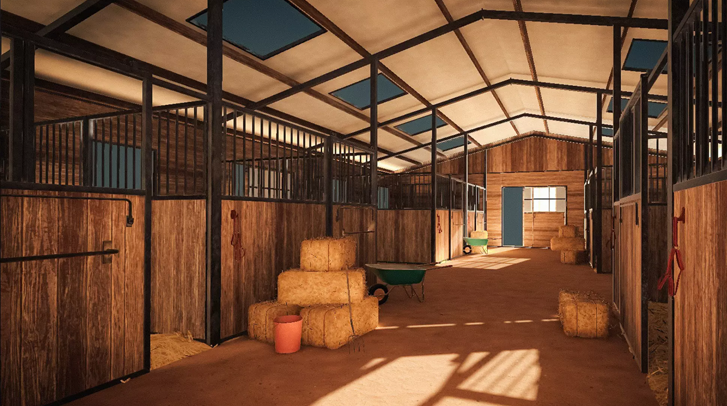
\includegraphics[width=0.32\textwidth]{images/unity-environments-stables.png}} 
%     \subfigure{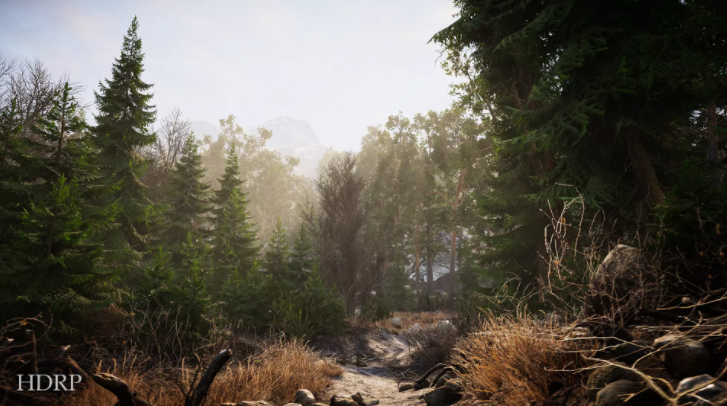
\includegraphics[width=0.32\textwidth]{images/unity-environments-forest.png}} 
%     \subfigure{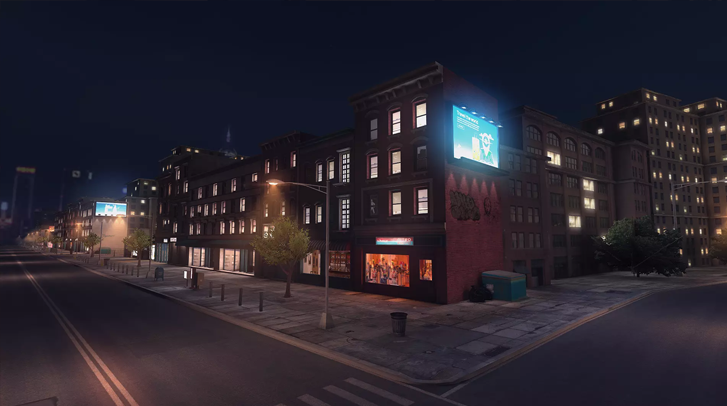
\includegraphics[width=0.32\textwidth]{images/unity-environments-city.png}}
%     \subfigure{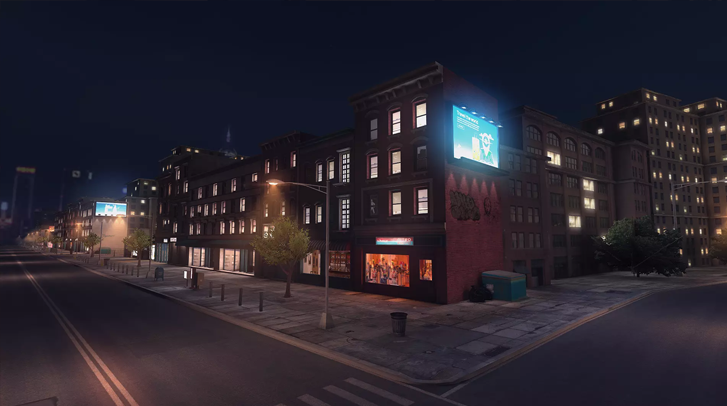
\includegraphics[width=0.32\textwidth]{images/unity-environments-city.png}}
%     \caption{Sample 3D assets for scenario proposals. Taken from \cite{unity-asset-store}.}
%     \label{fig:unity-my-3d-envs}
% \end{figure}

\begin{figure}[!ht]
    \centering
    \subfigure[Dreamscape Scenario.]{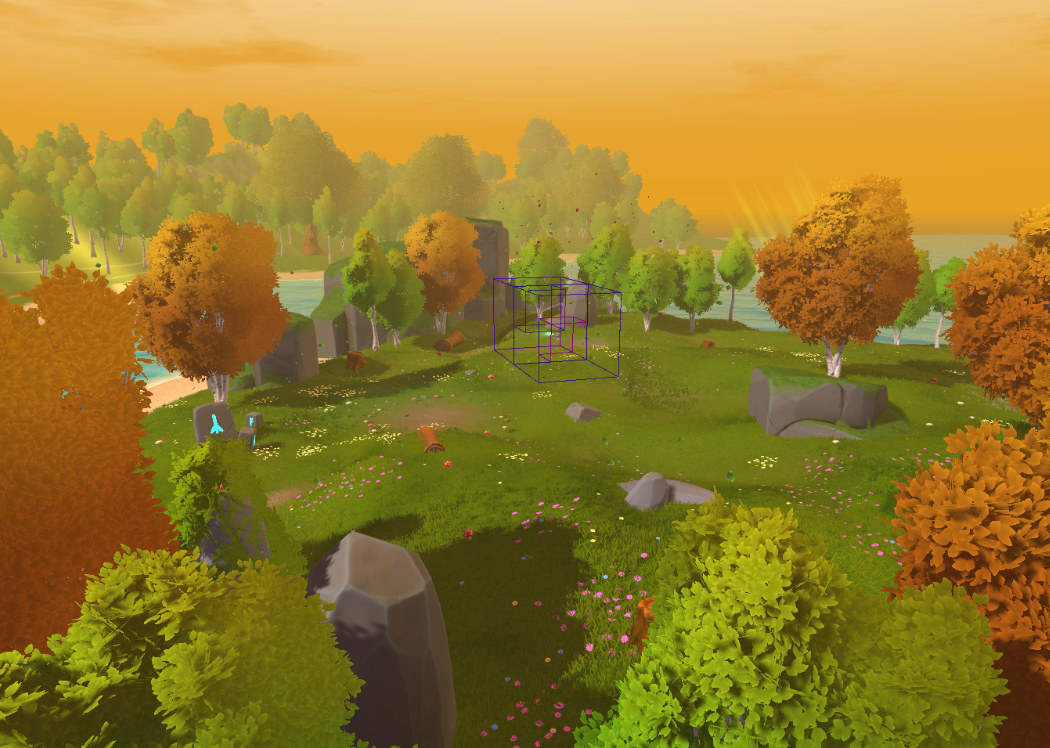
\includegraphics[width=0.245\textwidth]{images/unity-env-dreamscape.png} } 
    \subfigure[City Neighborhood.]{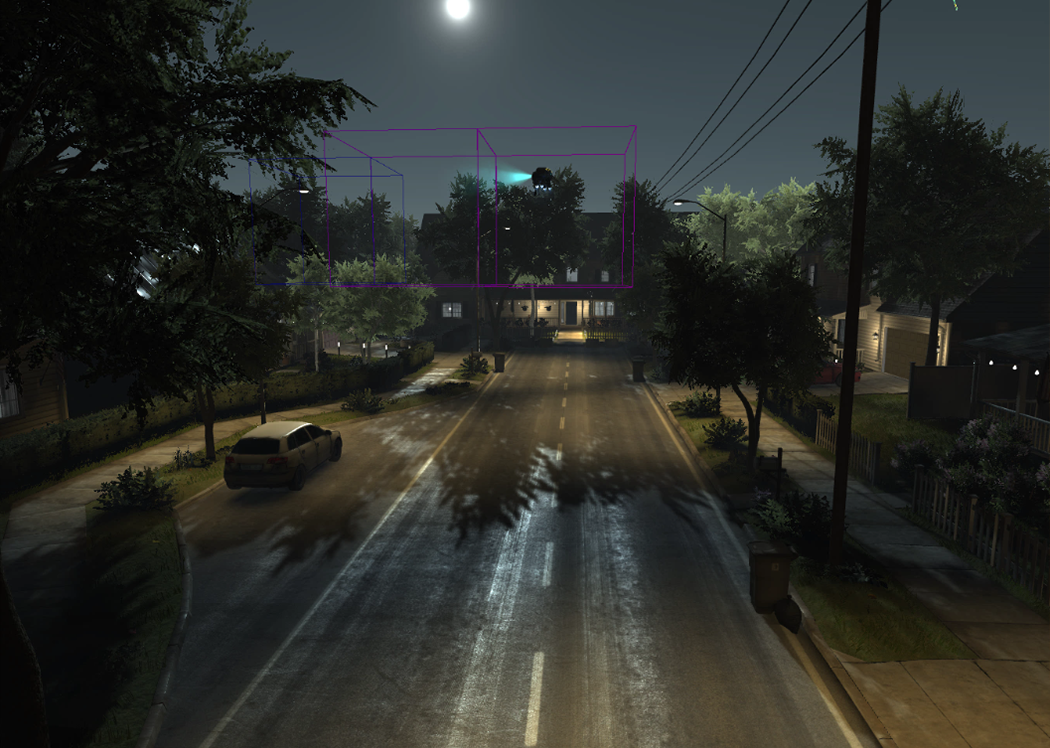
\includegraphics[width=0.245\textwidth]{images/unity-env-neighborhood.png}} 
    \subfigure[Snowy Forest.]{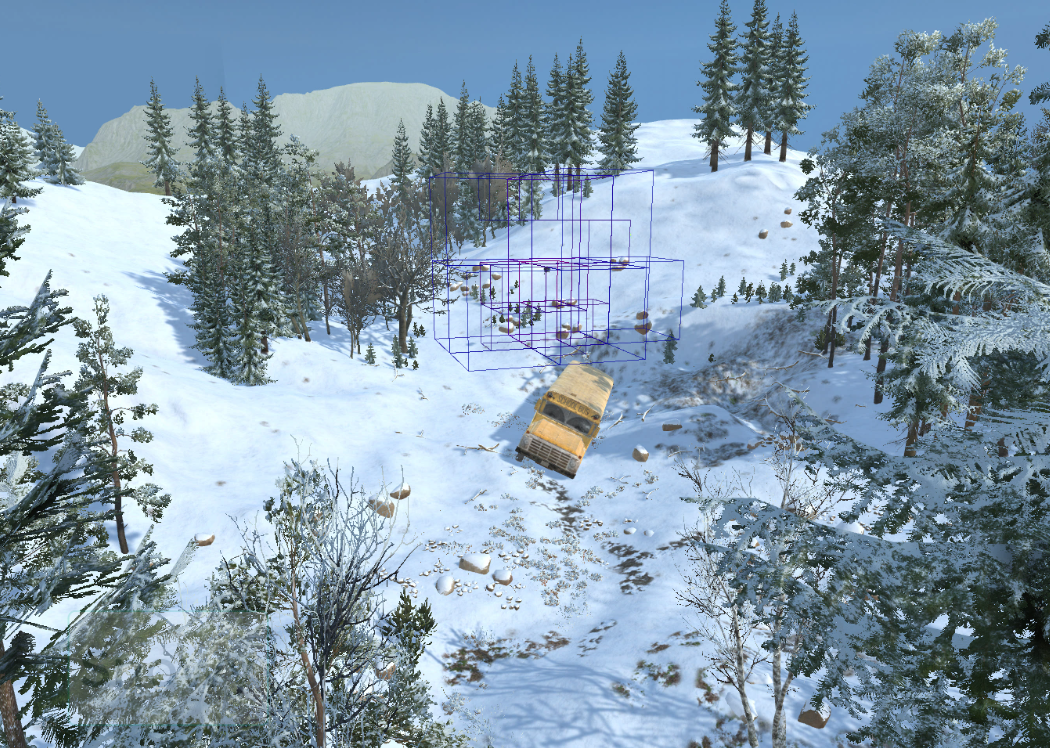
\includegraphics[width=0.245\textwidth]{images/unity-env-forest-snowy.png}}
    \subfigure[Summer Forest.]{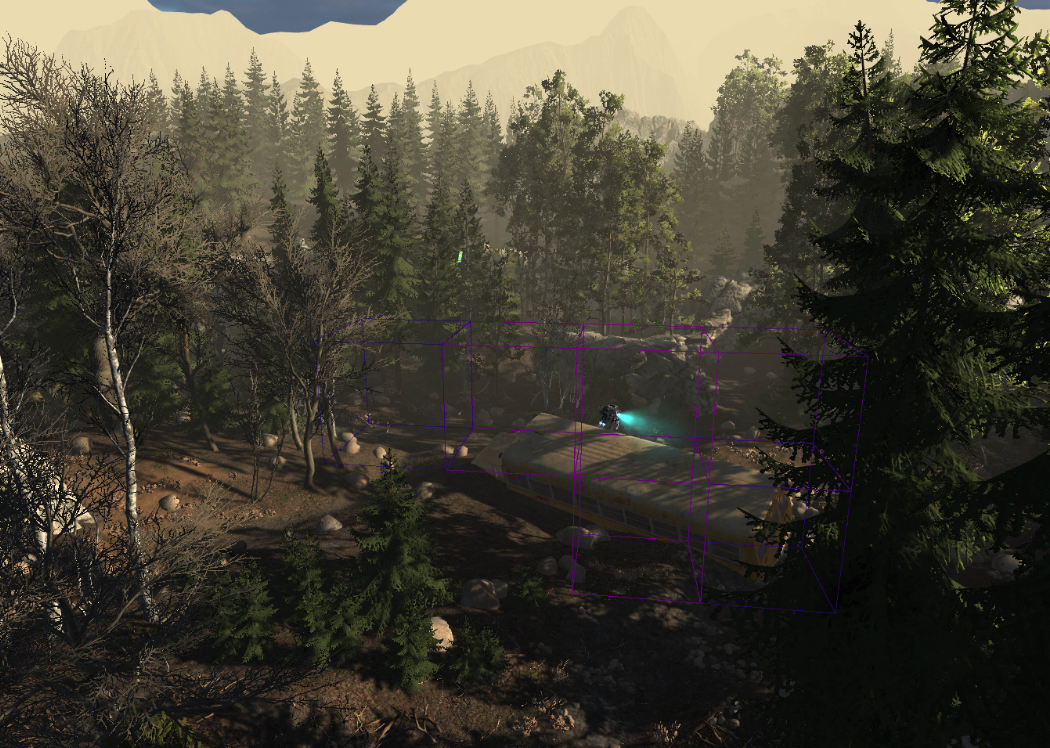
\includegraphics[width=0.245\textwidth]{images/unity-env-forest.png}}
    \caption{
        Modelled 3D scenarios to present the practical aspect of the proposed methods. 
        \\ 3D models subject to copyright from \textcite{unity-asset-store}.
    }
    \label{fig:unity-my-3d-envs}
\end{figure}

% \begin{figure}[!ht]
%         \centering
%         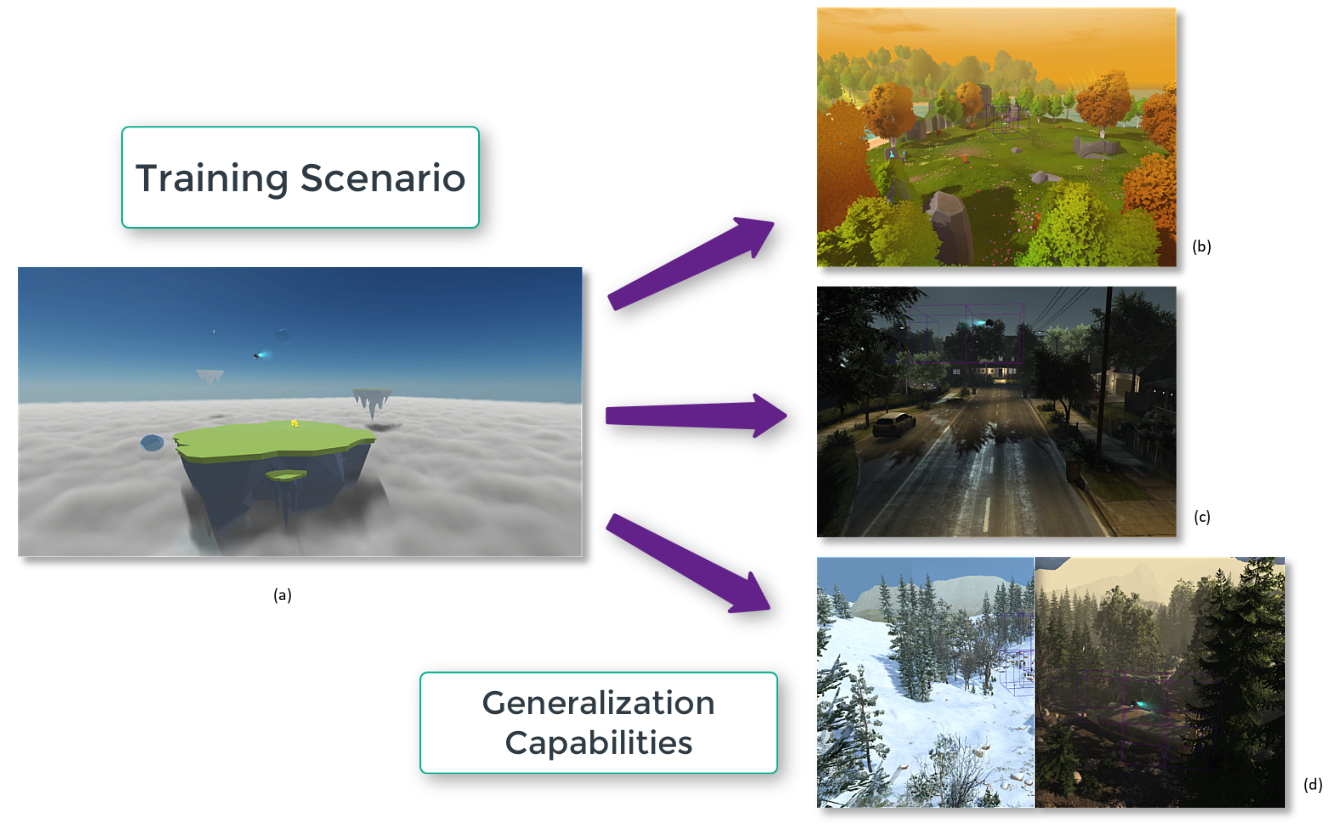
\includegraphics[width=0.6\textwidth]{images/unity-env-scenarios2.png}
%         \caption{Research Scenarios results.}
%         \label{fig:unity-simple-encoder}
% \end{figure}


Multiple 3D scenes have been collected and setup to demonstrate the applicability of our method in practical real world scenarios. Given the time constraint, deeper demonstrations of these specific use cases are out of scope.
% need to be modelled and constructed to demonstrate the applicability of the learned behavior across a variety of scenarios. 
Figure \ref{fig:unity-my-3d-envs} illustrates the training environment and different environments which were used to demonstrate the octree explorer agent's versatility to multiple environments.

\newpage
Concretely, the 3D environments that were used to test the portability of our approach are: 
\begin{itemize}
    \item \textbf{Dreamscape.} A fantasy forest scene.
    % in reference to the milking robot scenario from our industry partner, Sutter Landtechnik GmbH (SLG).
    \item \textbf{Forest.} An open nature scene with obstacles and a bus that was drove off as part of an accident. It is presented in three weathers: sunny, snowy and snowy overcast.
    \item \textbf{City Neighborhood.} A city scene where fires could be prevented with firefighter drones.
    % that presents buildings and rooms to navigate and explore.
\end{itemize}

Similarly , the voxel-curious agent showed visual agnostic performance to other voxelized objects such as bus and house, which are part of the environments above. 
% Finally, \textit{quidditch} goalposts were also used to test knowledge transferability.


% \subsection{Cross-Scenario Performance}

% The agent showed visual agnostic performance for our agent that was trained on a voxelized bicycle and then tested on a voxelized bus and voxelized house. Moreover, an additional \textit{quidditch} scene was tested, and the agent X showed the best cross-scenario performance. Below are the metrics collected for the cross-scenario performance:

% X

\subsection{Cross-Platform Compatibility}\label{chap:4:cross-platform-compatibility}
This section presents the results of the metrics determined to evaluate the effort of transferring the Unity ML-Agents environment to an OpenAI Gym compatible implementation. We define a compatible implementation as one that is ready to be trained and produce relevant results. The metrics are displayed in Table \ref{tab:results-cross-platform}.

\begin{longtable}{|l|c|}                            \hline
    \textbf{Metric}            
    & \thead{Value}  
    \\ \hline
    % portability of the training and the evaluation pipeline

    Lines of code                                       & ~1500                          \\ \hline
    Time required to transition the environment             & ~4h                           \\ \hline
    Time required to integrate to WandB                     & ~20h                       \\ \hline
    Time required to implement resuming of experiments       & ~40h                        \\ \hline
    Time required for other features                        & ~40h                        \\ \hline
    Agent reward after 10M timesteps (baselines)                    & -300                        \\ \hline
    Agent reward after 10M timesteps (mlagents)                    & -374                       \\ \hline
    \caption{Overview of cross-platform effort measurement metrics. The agent reward is reported for the training of the \textit{voxel-agent++100}. It is negative given that the the voxel rewards are sparse and the movement speed and lingering penalties are dense signals.}
    \label{tab:results-cross-platform}
\end{longtable}



% \begin{figure}
% \includegraphics[width=1.0\linewidth]{figs/results-on-robots-tutorial/sacs-performance.pdf}
% \caption{Performance comparison of the PPO, SAC, and a vanilla RL agent.}
% \label{fig:sacs-performance}
% \end{figure}





% Table \ref{tab:test-results} provides a brief summary of the results and the general performance of the used algorithms, which are discussed afterwards in more detail.
% \newpage

% \begin{longtable}
% {@{} l c c @{}} \toprule
% \textbf{Method}                     & \textbf{Accuracy}     & \textbf{Standard Deviation}       \\ \midrule
% % PCA                                 & 97\%                  & 0.015                             \\ \midrule
% MAV                                 & \textbf{97\% }                 & \textbf{0.43}                             \\ \midrule
% DOPE                                & 0\%                  & -                             \\ \midrule
% RANSAC                              & 0\%                   & -                             \\ \bottomrule
% \caption{Statistics of tested methods.} \label{tab:test-results}                          \\
% \end{longtable}

% The following Table \ref{tab:DOPE-results} displays the results for the DOPE algorithm. DOPE uses FAT formatted data sets, which are generated using NDDS, in Unreal Engine 4. These data sets are characterized for being synthetic photorealistic images. The data set variants presented below are optimized by modifying the parameters in data set used, such as:
% % The variants used include changes in: 
% the realism degree in the materials used for the object textures, the usage of rotation in the focus object, and the usage of obstructive objects. Aditionally, all data sets include five different photorealistic scenes: beach, studio, temple, meadow and zen garden. Surprisingly none of the data sets were realistic enough to close the reality gap, which reflected in DOPE not outputting any predictions.



% \begin{longtable}{|l|c||c|}                            \hline
% \multicolumn{3}{|l|}{\textbf{Deep Object Pose}}              \\\hline
% \textbf{Dataset}            & \textbf{Size}  & \textbf{Functional}            \\ \hline
% NDDS Photorealistic (base)       & 260k      & No                             \\ \hline
% NDDS with Rotation          & 80k       & No                             \\ \hline
% NDDS Small                  & 20k       & No                             \\ \hline
% \caption{Overview of the best DOPE results for the respective dataset variations.} \label{tab:DOPE-results}
% \end{longtable}


% The results for the RANSAC algorithm are shown in Table \ref{tab:ransac-results}. The skimage implementation was used for both RANSAC and direct ORB matching. The variants presented were surprinsingly not succesful at matching X. It is suspected that RANSAC and ORB matching are not the best approach for identifying simple texture objects such as the cow teats. 
% Figure \ref{fig:ransac-results} illustrates the suspicion and the behavior of RANSAC on both the RGB and the depth images. RANSAC was tested by varying the ORB number of keypoints, the ORB threshold and RANSAC's residual threshold as well as adding a denoising step.  


% \begin{longtable}{|c|c|c|c||c|}                            \hline
% \multicolumn{5}{|l|}{\textbf{RANSAC / ORB Matching}}              \\\hline
% \textbf{ORB \#keypoints} & \textbf{ORB threshold} & \textbf{Residual Threshold} & \textbf{Denoising}       & \textbf{Functional}      \\ \hline
%         20      & 0.08      & N/A (ORB matching)       & No     &  No               \\ \hline
%         200     & 0.08      & N/A (ORB matching)       & No     &  No               \\ \hline
%         200     & 0.02      & 0.5       & No     &  No               \\ \hline
%         200     & 0.02      & 0.5       & Yes    &  No               \\ \hline
%         200     & 0.02      & 0.9       & No     &  No               \\ \hline
%         200     & 0.02      & 0.9       & Yes    &  No               \\ \hline
%         200     & 0.08      & 0.5       & No     &  No               \\ \hline
%         200     & 0.08      & 0.5       & Yes    &  No               \\ \hline
%         200     & 0.08      & 0.9       & No     &  No               \\ \hline
%         200     & 0.08      & 0.9       & Yes    &  No               \\ \hline
% \caption{Overview of the best MAV results for the respective offset-averaging mechanisms combinations.} \label{tab:ransac-results}                          
% \end{longtable}


%  \begin{figure}[h]
%         \centering
%         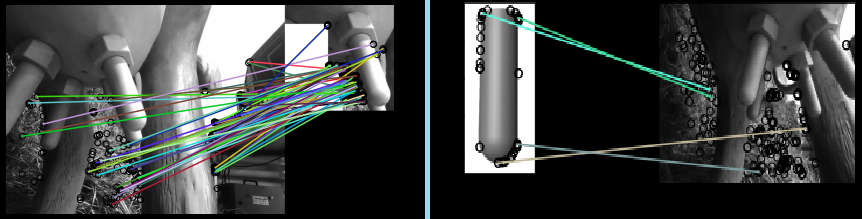
\includegraphics[width=0.9\textwidth]{images/cow_ransac.png}
%         \caption{RANSAC's behavior on the cow data set.}
%         \label{fig:ransac-results}
%     \end{figure}
    
% The following table 
% % \ref{tab:mav-results} displays 
% presents the results for the "MAV" algorithm. The optimizations presented are a combination of the offset and the averaging method.

% \begin{longtable}{|l|l||c|c|c|}                                              \hline
% \multicolumn{5}{|l|}{\textbf{MAV}}                                                       \\\hline
% \textbf{Offset}         & \textbf{Averaging Method}   
% & \textbf{Average Error}  & \textbf{Standard Deviation}  & \textbf{Execution Time}                 \\ \hline
% Fixed                   & Single Point                & 1.13            & 2.8              & 0.26 - 1.5 secs   \\ \hline
% Calculated              & Single Point                & 1.77            & 3.3              & 0.26 - 1.5 secs   \\ \hline
% Fixed                   & Average: 1/3rd              & \textbf{0.67}   & \textbf{2.4}     & 0.26 - 1.5 secs                     \\ \hline
% Calculated              & Average: 1/3rd              & 1.54            & 2.93             & 0.26 - 1.5 secs    \\ \hline
% Fixed                   & Average: 1/10th             & 0.96            & 2.55             & 0.26 - 1.5 secs     \\ \hline
% Calculated              & Average: 1/10th             & 1.51            & 2.87             & 0.26 - 1.5 secs    \\ \hline
% \caption{Overview of the best MAV results for the respective offset-averaging mechanisms combinations.} \label{tab:mav-results}                          
% \end{longtable}

% \subsubsection{Research Question 2}

% The second research question tackles the evaluation of the pose estimation of cow teats.

% \subsubsection{Quality Ranking of Predictions}


\section{Deliverables}
The following deliverables will be handed in with this master thesis:
\begin{itemize}
    \item This work produced three types of exploration-capable agents: environment-focused, object-focused and mixed-focused.
    The environment-focused agent is able to explore twice as many leaf nodes as the non-explorative models (71 versus 35 average leaf nodes per episode). This means that the average performance of the explorative agent explores 88\% of the small environment. 
    
    \item  The object-focused agent is able to scan at least 2 objects per episode on average. This translates to a scanning speed of 2500 time steps per object.
    
    \item Finally, the mixed exploration agent is able to keep up with the 2 objects per episode performance and explore an average 41 leaf nodes per episode, which covers 51\% of the environment, outperforming the 43\% coverage of object-focused models.
   
   \item A set of baselines are also handed in, used to analyze the performance of traditional methods for exploration (random actions, shortest path) and other state-of-the-art-inspired methods (object detection maximization, semantic curiosity, semantic entropy).
   
    \item The trained models for our proposed method in ONNX formats, including all other variants for voxel and octree exploration and an out-of-the-box Unity-ready reinforcement learning environment capable of reproducing the experiments and results.

    \item For future research, a set of Unity scenes that demonstrate the versatility of the reinforcement learning agent. These scenes further allow the creation of future benchmarks for other synthetic data models and use cases, which are not limited to machine learning approaches.
\end{itemize}
